\chapter{基于传统机器学习方法的低分辨率环境下微表情识别}\label{chap:owner1}

微表情是一种基本的非言语行为,可以忠实地表达人类隐藏的情感。它在国家安全、计算机辅助诊断等领域有着广泛的应用,鼓励我们开展微表情自动识别的研究。然而,从监控视频中获取的图像容易出现质量低下的问题,给实际应用带来困难。由于所捕获图像的质量较低,现有的算法无法达到预期的效果。针对这一问题,我们对面部幻觉法在低分辨率情况下的微表情识别问题进行了全面的研究。实验结果表明,该框架在低分辨率情况下的微表情识别中取得了良好的效果。

目前的微表情识别算法虽然取得了较为合理的效果,但其性能在很大程度上取决于人脸视频剪辑的质量。一旦用于识别的人脸视频片段质量较差(如分辨率较低),上述算法就无法正常工作。原因主要有两个方面:(1)低分辨率图像丢失了大量的细节信息,导致从低分辨率图像序列中提取可用特征的困难\citep{lei2011local}。(2)低分辨率图像与高分辨率图像(如不同分辨率、不同清晰度)不一致,导致我们在测试阶段无法直接使用低分辨率图像作为输入。在现实世界中,从监控录像中获取的面部图像通常只占整个画面的一小部分。例如,用于微表情识别的SMIC数据集的面部分辨率为$190\times230$。然而,监控视频捕捉到的面部图像序列的分辨率往往在$50\times50$(或更低)以下。这意味着以前的微表情识别方法不能直接用于处理低分辨率的情况。因此,低分辨率情况下的微表情识别研究具有重要意义和挑战性。

为了解决上述问题,我们利用最近的面部幻觉方法进行了低分辨率微表情识别的研究。我们首先对低质量的人脸图像序列产生幻觉,以恢复丢失的动态特征。然后,我们采用传统的微表情识别方法来探索低质量的微表情识别。我们评估了不同分辨率下微表情识别准确率的表现,研究了分辨率与识别准确率之间的关系。一般来说,本文的目标是全面研究分辨率对微表情识别的影响,同时开发一个框架来处理低质量条件下的微表情识别任务。

低分辨率微表情识别过程包括图像序列预处理、超分辨率重建、特征提取和分类,如图~\ref{fig10}所示。详细描述如下:

\begin{figure}[!htbp]
    \centering
    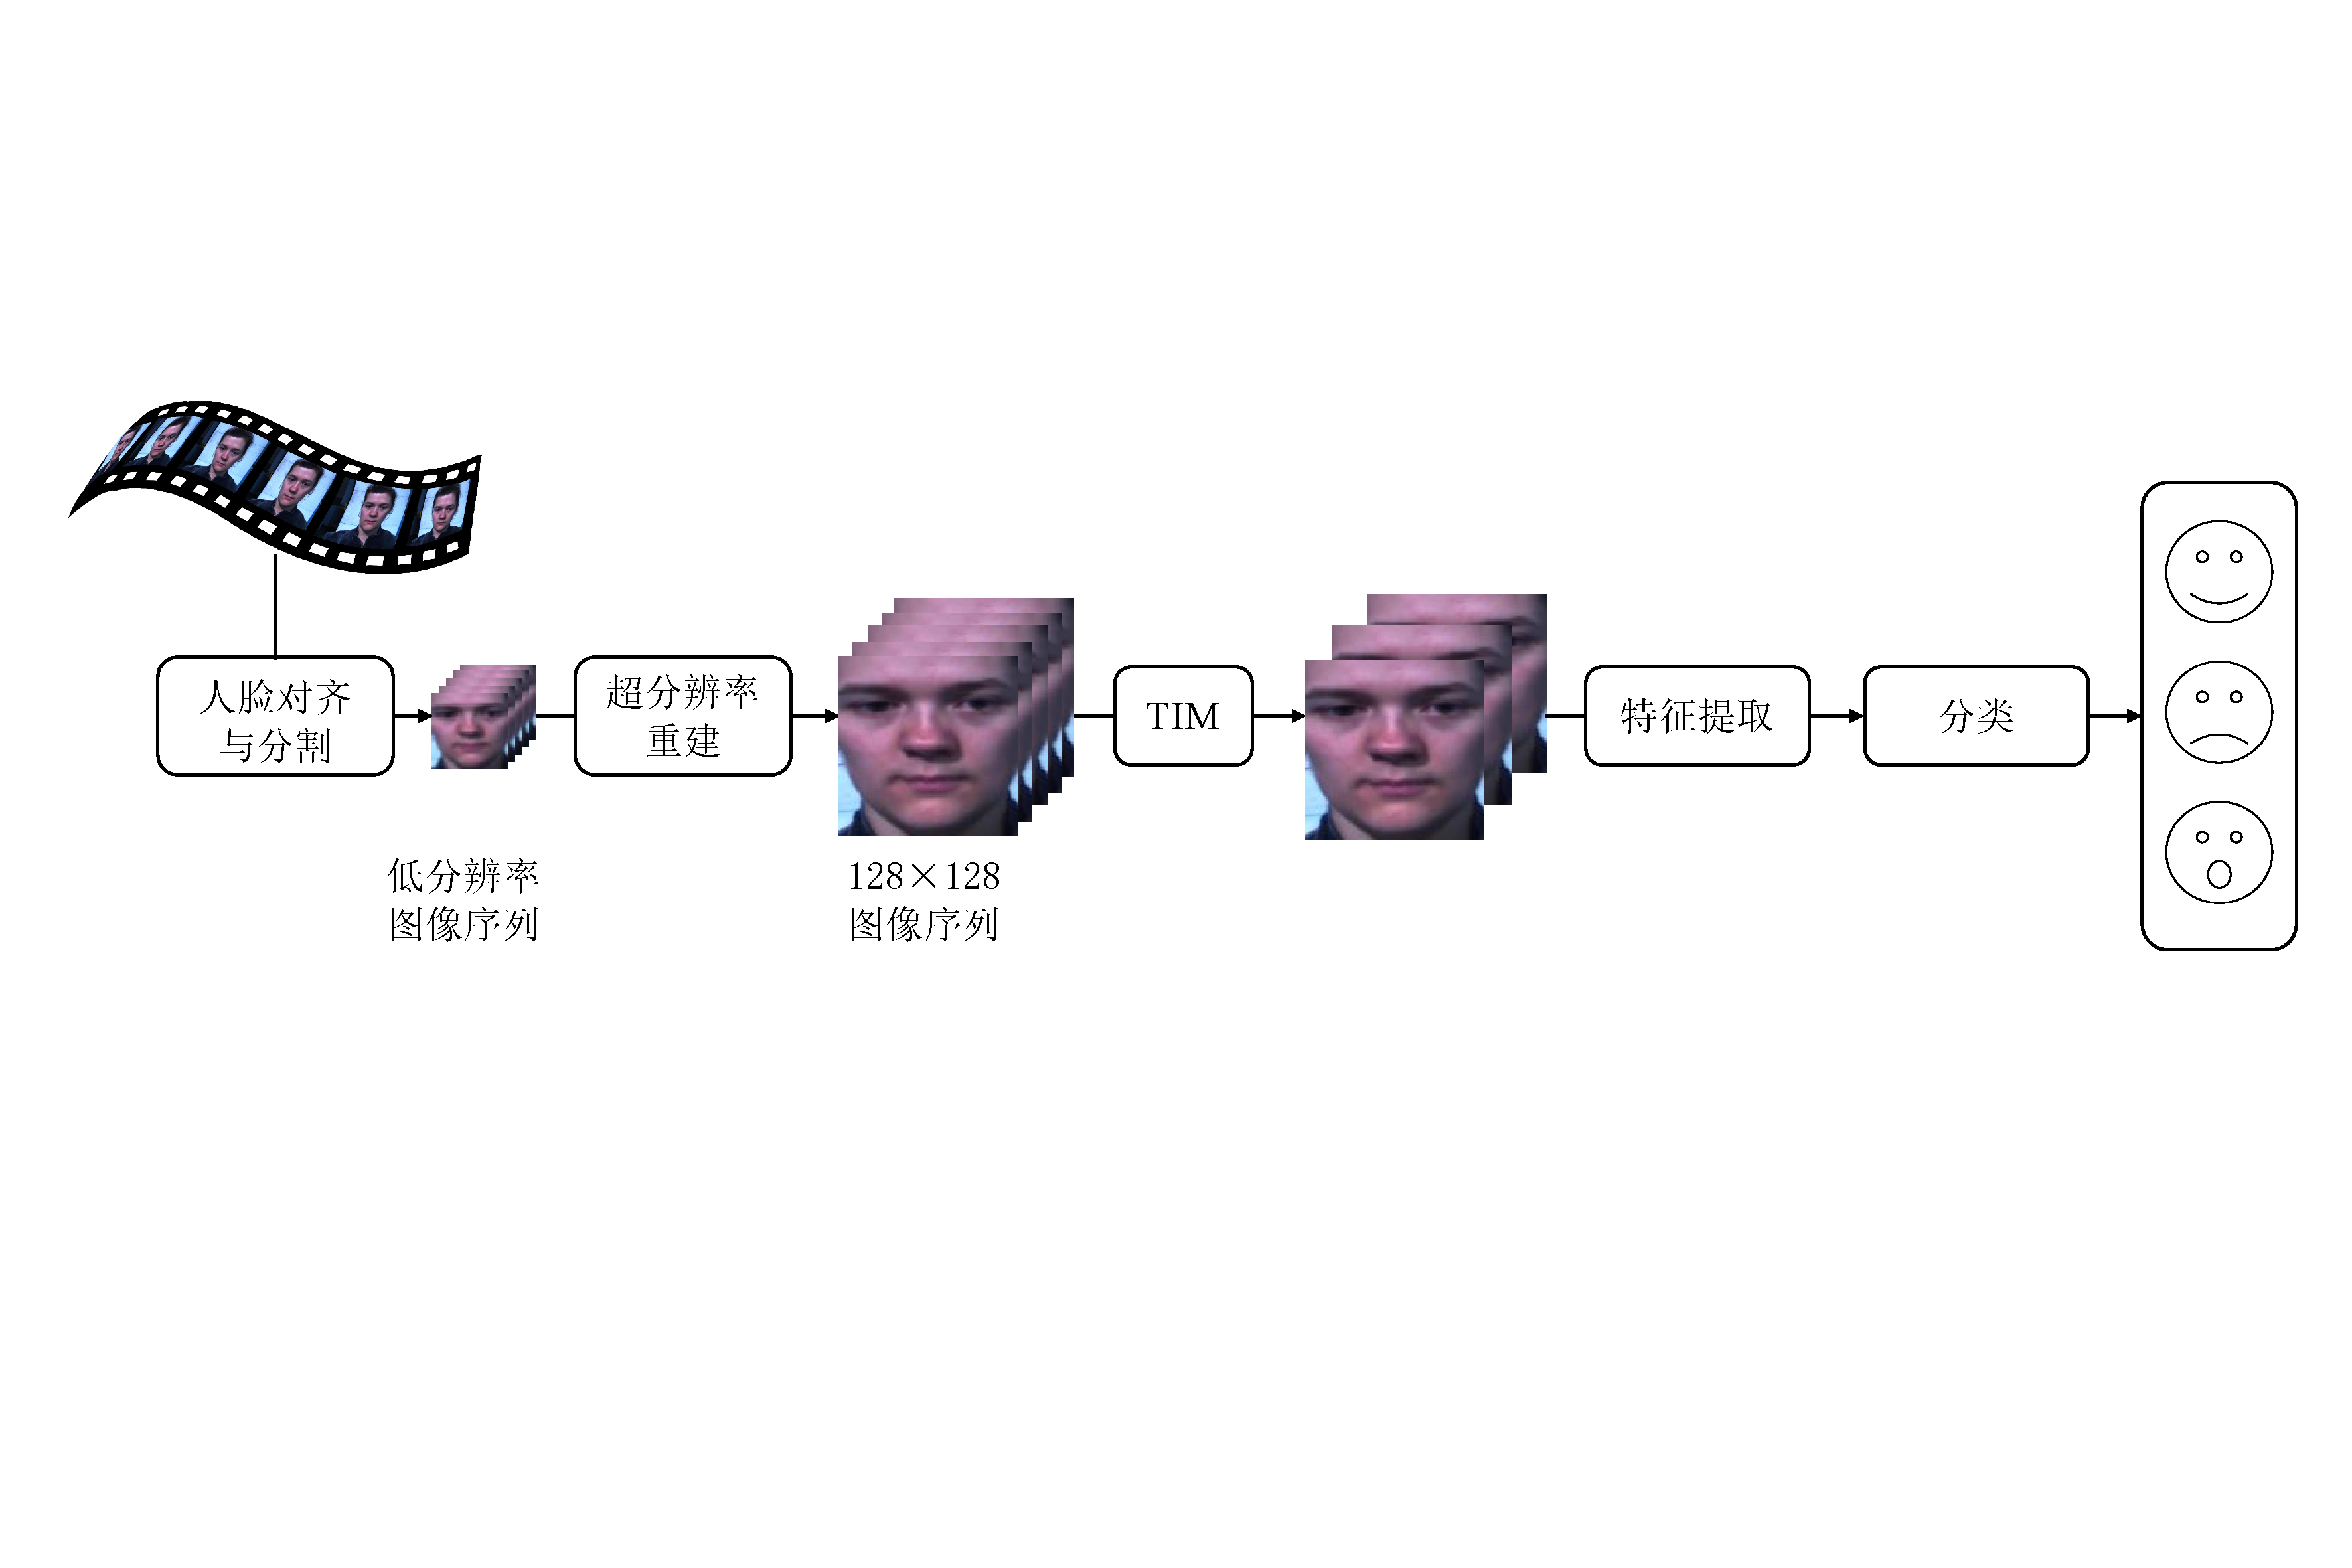
\includegraphics[width=0.95\textwidth]{LR0}
    \caption{低分辨率环境下微表情识别框架}
    \label{fig10}
\end{figure}

\section{低分辨率微表情数据获取}

微表情识别的数据集有很多,如SMIC和CASME II。然而,这些数据集都是专业相机在特定环境下获取的高清图像序列。图~\ref{fig11}显示了SMIC-HS数据集的视频片段中的两帧。我们可以在红色框中发现面部表情的细微变化。特别是白色椭圆区域的运动和白色箭头的位置更为明显。如果图像分辨率太低,这些细节很难被注意到。

\begin{figure}[!htbp]
\centering
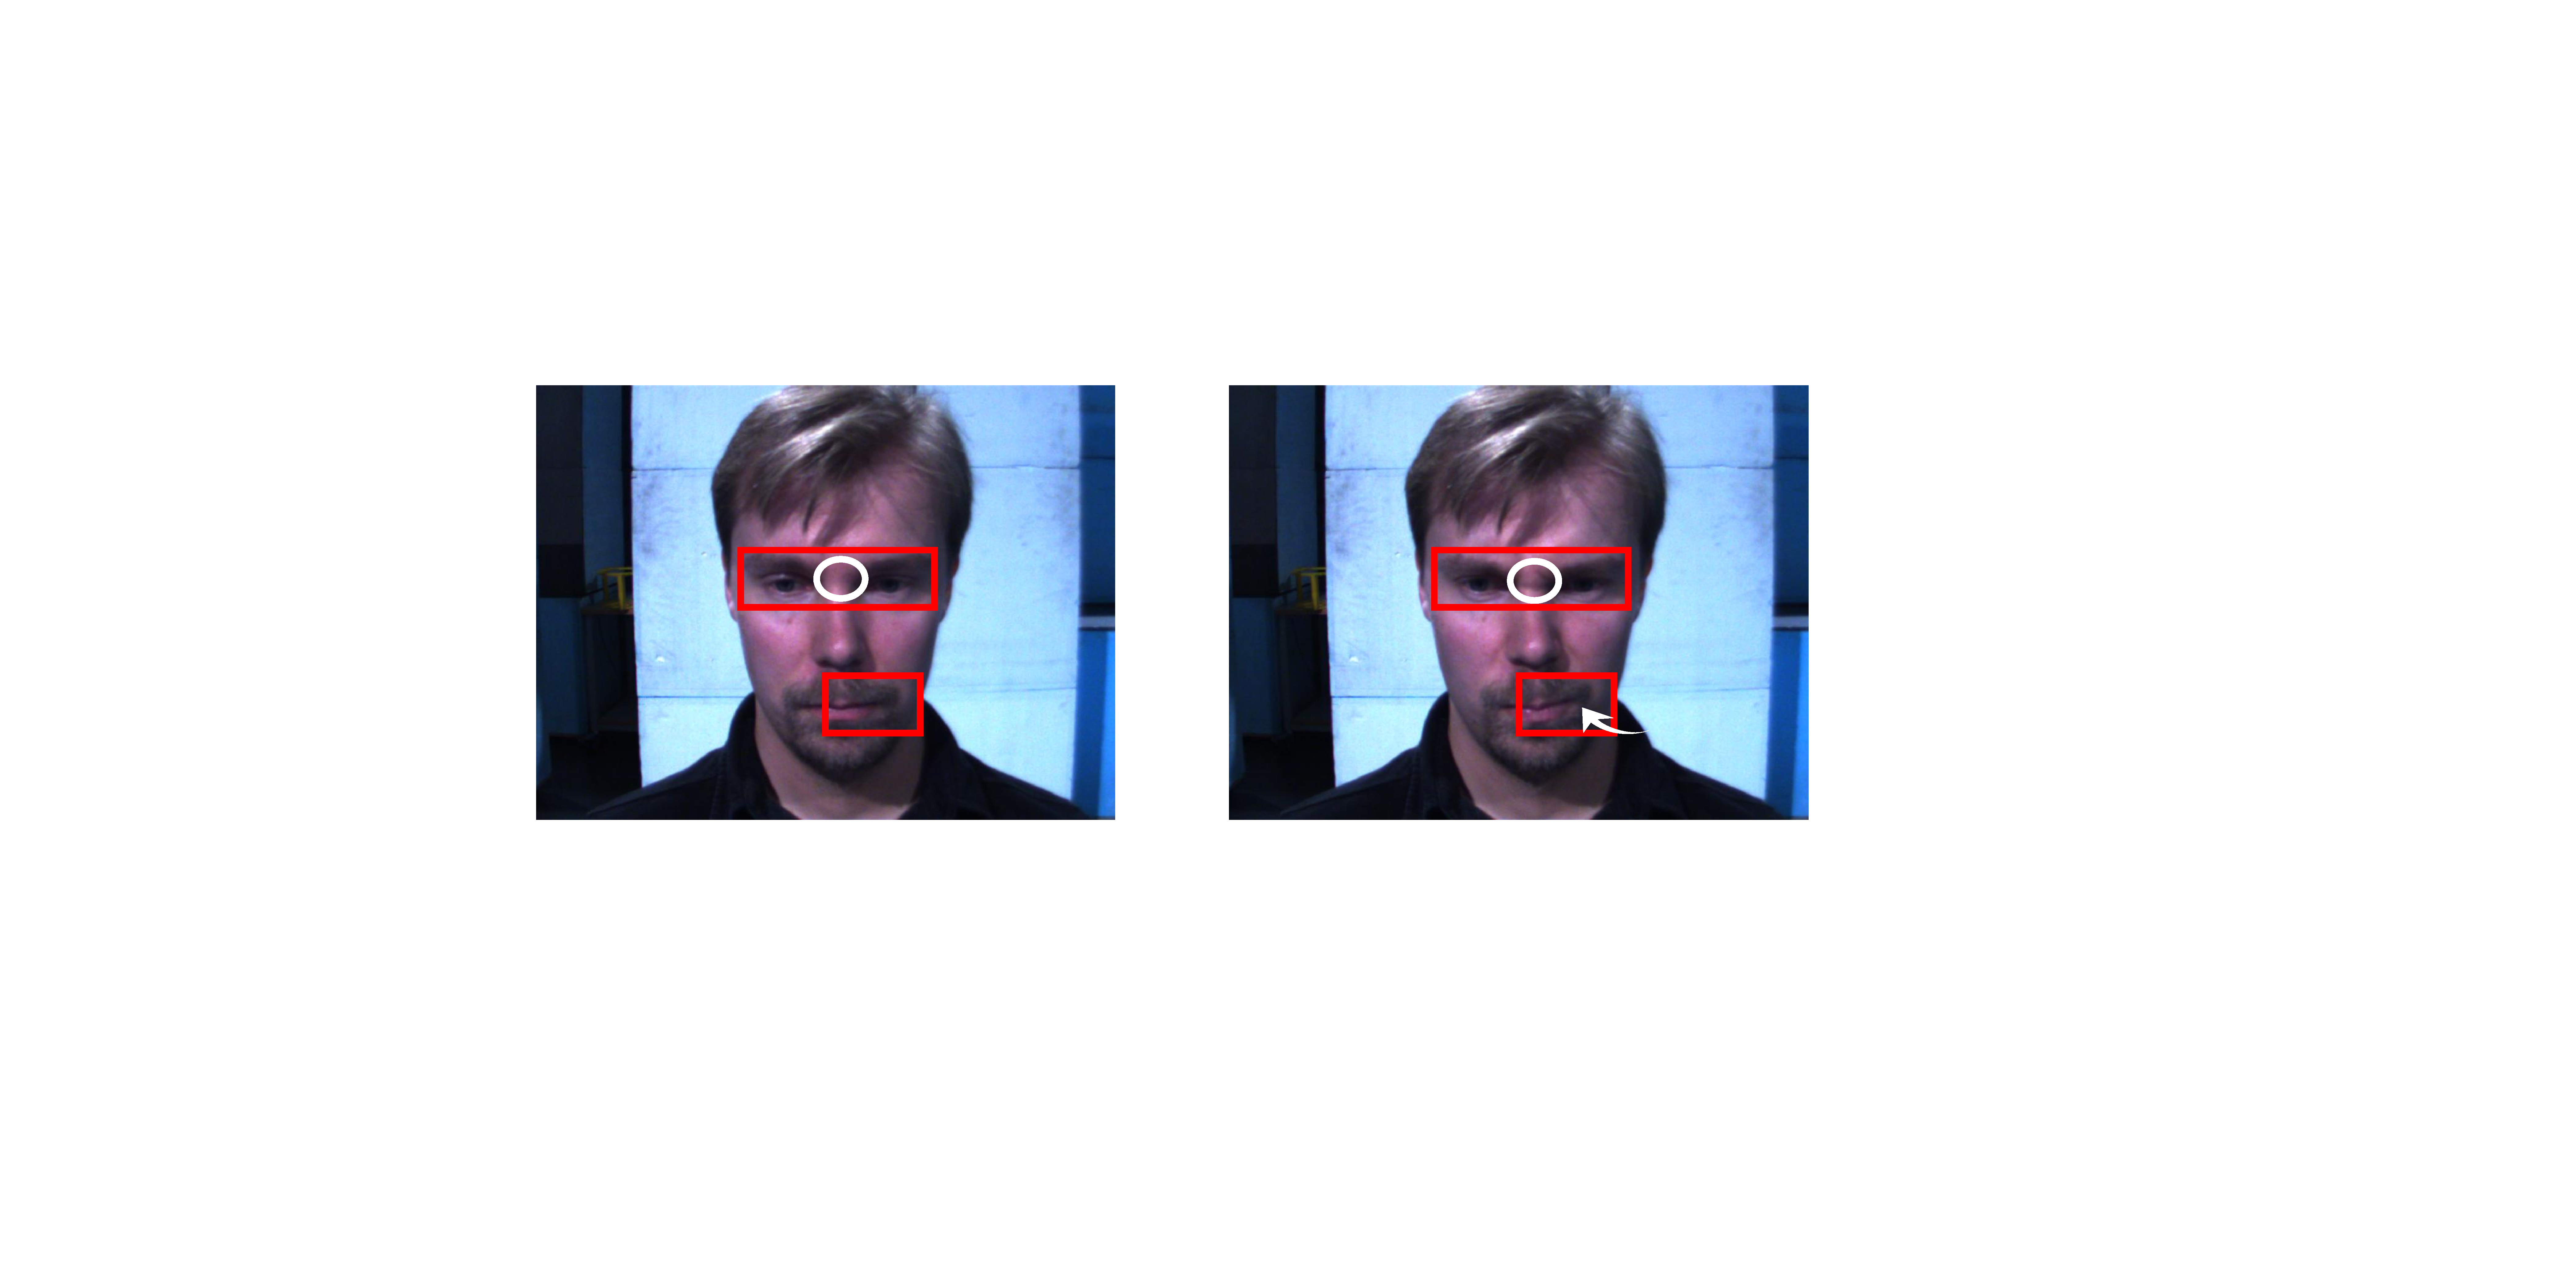
\includegraphics[width=0.65\textwidth]{LR1}
\caption{来自SMIC-HS数据集的两帧}
\label{fig11}
\end{figure}

由于现有的自发微表情数据集中不存在低分辨率的图像序列,我们采用图像恶化处理的方法来获得模拟的低分辨率的微表情图像序列。本文将低分辨率图像分为三大类:小尺寸、低质量和小尺寸放大器、质量较差\citep{wang2014low}。我们考虑第三种类型的图像(小尺寸、质量差),即更接近真实应用的情况,如模拟图像。

在图像重建任务中,低分辨率图像序列是通过对高分辨率图像序列进行模糊、下采样和噪声处理得到的\citep{shi2018hallucinating}:
\begin{equation}
    \label{eq1}
    \boldsymbol{L} = \boldsymbol{DBH}+\boldsymbol{n}
\end{equation}
其中 $\boldsymbol{D}$和$\boldsymbol{B}$分别是下采样和模糊处理,$\boldsymbol{H}$是高分辨率图像,$\boldsymbol{n}$是加性噪声,$\boldsymbol{L}$是低分辨率图像。

\section{数据预处理}

在我们提出的框架中,预处理主要包括三个步骤:人脸对齐、人脸分割和TIM。原始视频中有自然的姿势变化和无意识的运动。同时,收集不同性别、年龄、种族的参与者的微表情视频片段。因此,为了避免上述非表达因子的干扰,进行人脸对齐和人脸分割是必不可少的。

Since MEs are very subtle, other differences (e.g., face size and face shape) between clips need to be minimized in order to reduce intra-class variations and highlight the inter-class differences generated by ME movements. For this purpose we align all faces to a model face in the following way.
由于MEs是非常细微的,为了减少类内变化和突出ME运动产生的类间差异,需要最小化剪辑之间的其他差异(如面大小和面形状)。为此,我们以以下方式将所有面与模型面对齐。

First, we select a neutral face image Imod as the model face. Sixty eight facial landmarks of the model face ψ(Imod) are detected using the Active Shape Model ( Cootes et al. 1995). For the ith ME clip, the 68 landmarks are detected on the first frame I1 Then we use the Local Weighted Mean (LWM) (Goshtasby 1988) to compute a transform matrix between the landmarks of I1 and Imod. The transform matrix T RAN is: T RANi, where ψ(Ii,1) is the coordinates of 68 landmarks of the first frame of the ME clip vi . All rest frames of this ME clip were normalized using matrix T RANi . The normalized image I 0 was computed as a 2D transformation of the original image: I1, where I1 is the jth frame of the normalized ME clip v1. At last, the face areas were cropped out from normalized images of each ME clip using a rectangular defined according to the eye locations in the first frame I1.
首先,我们选择一个中性的人脸图像Imod作为模型人脸。六十八面部地标模型的脸ψ(Imod中)发现使用主动形状模型(傻瓜et al . 1995年)。对于第i个ME片段,在第一帧I1上检测到68个地标,然后使用局部加权平均(LWM) (Goshtasby 1988)计算I1和Imod地标之间的变换矩阵。变换矩阵T跑:T王妃,ψ(2,1)的坐标68地标的第一帧我剪辑vi。该ME剪辑的所有静止帧均使用矩阵T RANi进行归一化。将归一化图像i0计算为原始图像I1的二维变换,其中I1为归一化ME clip v1的第j帧。最后,根据第一帧I1中眼睛位置定义的矩形,从每个ME剪辑的归一化图像中裁剪出人脸区域。

\subsection{主动形状模型}

我们从一个特定的片段中选取一个正面和中性表情的帧作为标准模板,手工定位两只眼睛的位置。然后,利用主动形状模型(Active Shape Model, ASM)检测68个面部地标\citep{cootes1995active}。利用局部加权平均(LWM)建立正则帧68个面部地标与其他帧68个面部地标之间的关系,将微表情图像与正则帧对齐,减少非表情因素的干扰\citep{goshtasby1988image}。

从采集的视频中选取其中没有表情且正面人脸的一帧作为模型脸$\boldsymbol{I_{mod}}$ ,应用ASM算法标定68个人脸关键点$\boldsymbol{\psi(I_{mod})}$,若错误标定其他物品或其他人脸(非主要人脸)时,计算任意对应位置关键点的相对距离$\boldsymbol{L(I_{mod})}$ :
\begin{equation}
    \label{eq2}
    \boldsymbol{L^{(i)}(I_{mod})}=\left \| \boldsymbol{\psi_{I_{mod}}}(p\pm 68)-\boldsymbol{\psi_{I_{mod}}}(q\pm 68) \right \|_{2}^{2\displaystyle }
\end{equation}
其中$i$指标定的关键点组数;$p$、$q$指一个关键点组中任意两点;$n$为关键点的个数,数量为68的倍数。选择相对距离$\boldsymbol{L^{(i)}(I_{mod})}$ 最大的一组关键点确定视频帧中主要人脸。如图~\ref{fig12}所示,1框内为主要人脸,2框为错误识别。

\begin{figure}[!htbp]
\centering
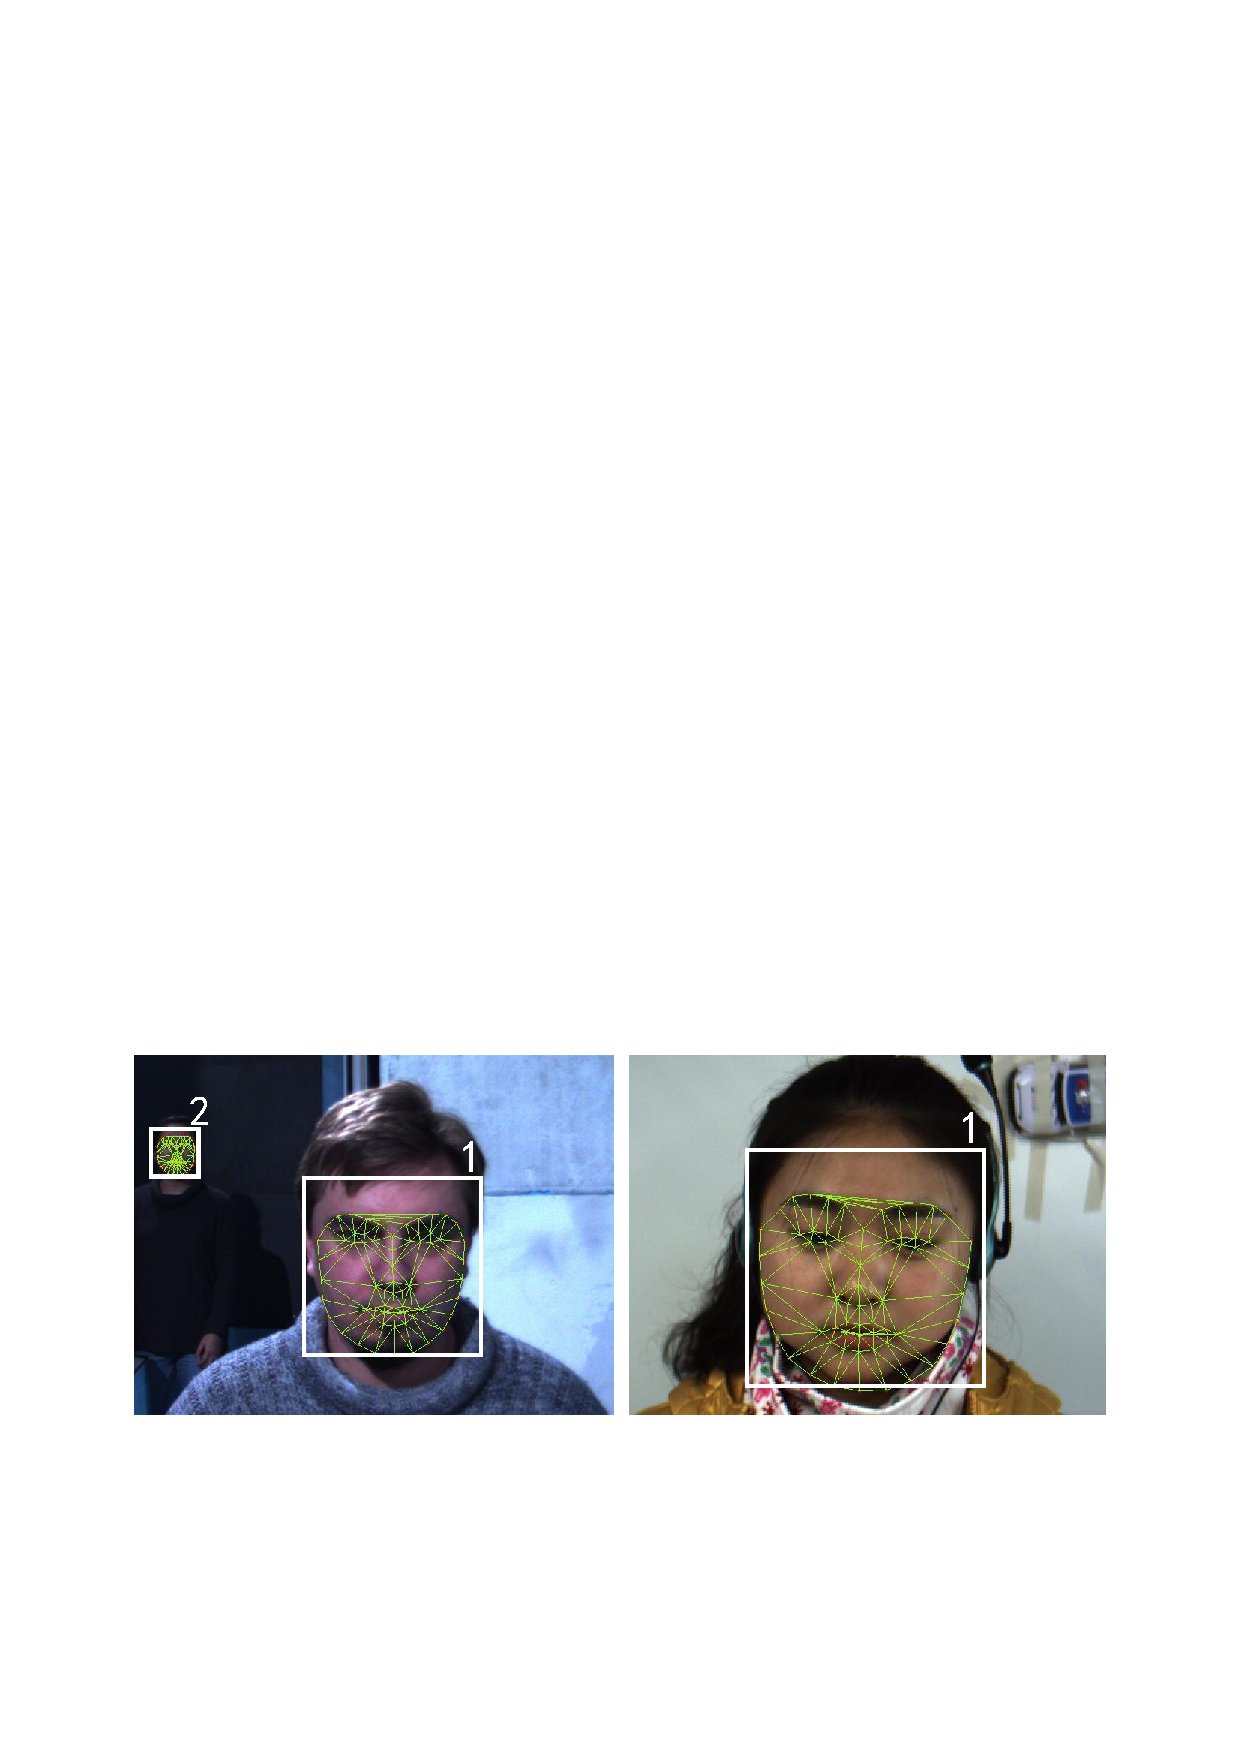
\includegraphics[width=0.65\textwidth]{3LR1}
\caption{ASM算法标定的68个人脸关键点}
\label{fig12}
\end{figure}

\subsection{局部加权平均算法}

对每段个视频的第一帧$\boldsymbol{I_{j,1}}$应用ASM算法标定68个人脸关键点$\boldsymbol{\psi (I_{j,1})}$,使用LWM函数建立模型脸关键点集$\boldsymbol{\psi (I_{mod})}$与视频第一帧关键点集$\boldsymbol{\psi (I_{j,1})}$之间的对应关系:
\begin{equation}
    \label{eq3}
    \boldsymbol{T_{j}}=LWM(\boldsymbol{\psi (I_{mod})},\boldsymbol{\psi (I_{J,1}))},~~j=1,\cdots ,l
\end{equation}
其中$j$是视频段号,$l$是视频片段总数。对视频片段的所有帧应用该关系,使视频的每一帧具有与模型脸$\boldsymbol{\psi (I_{mod})}$统一的姿态:
\begin{equation}
    \label{eq3}
    \boldsymbol{I_{j,k}^{'}}=\boldsymbol{T_{j}}\times \boldsymbol{I_{j,k}},\quad k=1,\cdots ,n_{j}
\end{equation}
其中$\boldsymbol{I_{j,k}}$为第$j$个视频片段的第$k$帧,$\boldsymbol{I_{j,k}^{'}}$为统一姿态后的第$j$个视频片段的第$k$帧,$n_{j}$为$j$视频片段的帧数。如图~\ref{fig13}所示,两图均按照模型脸统一姿态,左图剔除了错误识别,右图改变了头部的倾斜角度。

\begin{figure}[!htbp]
\centering
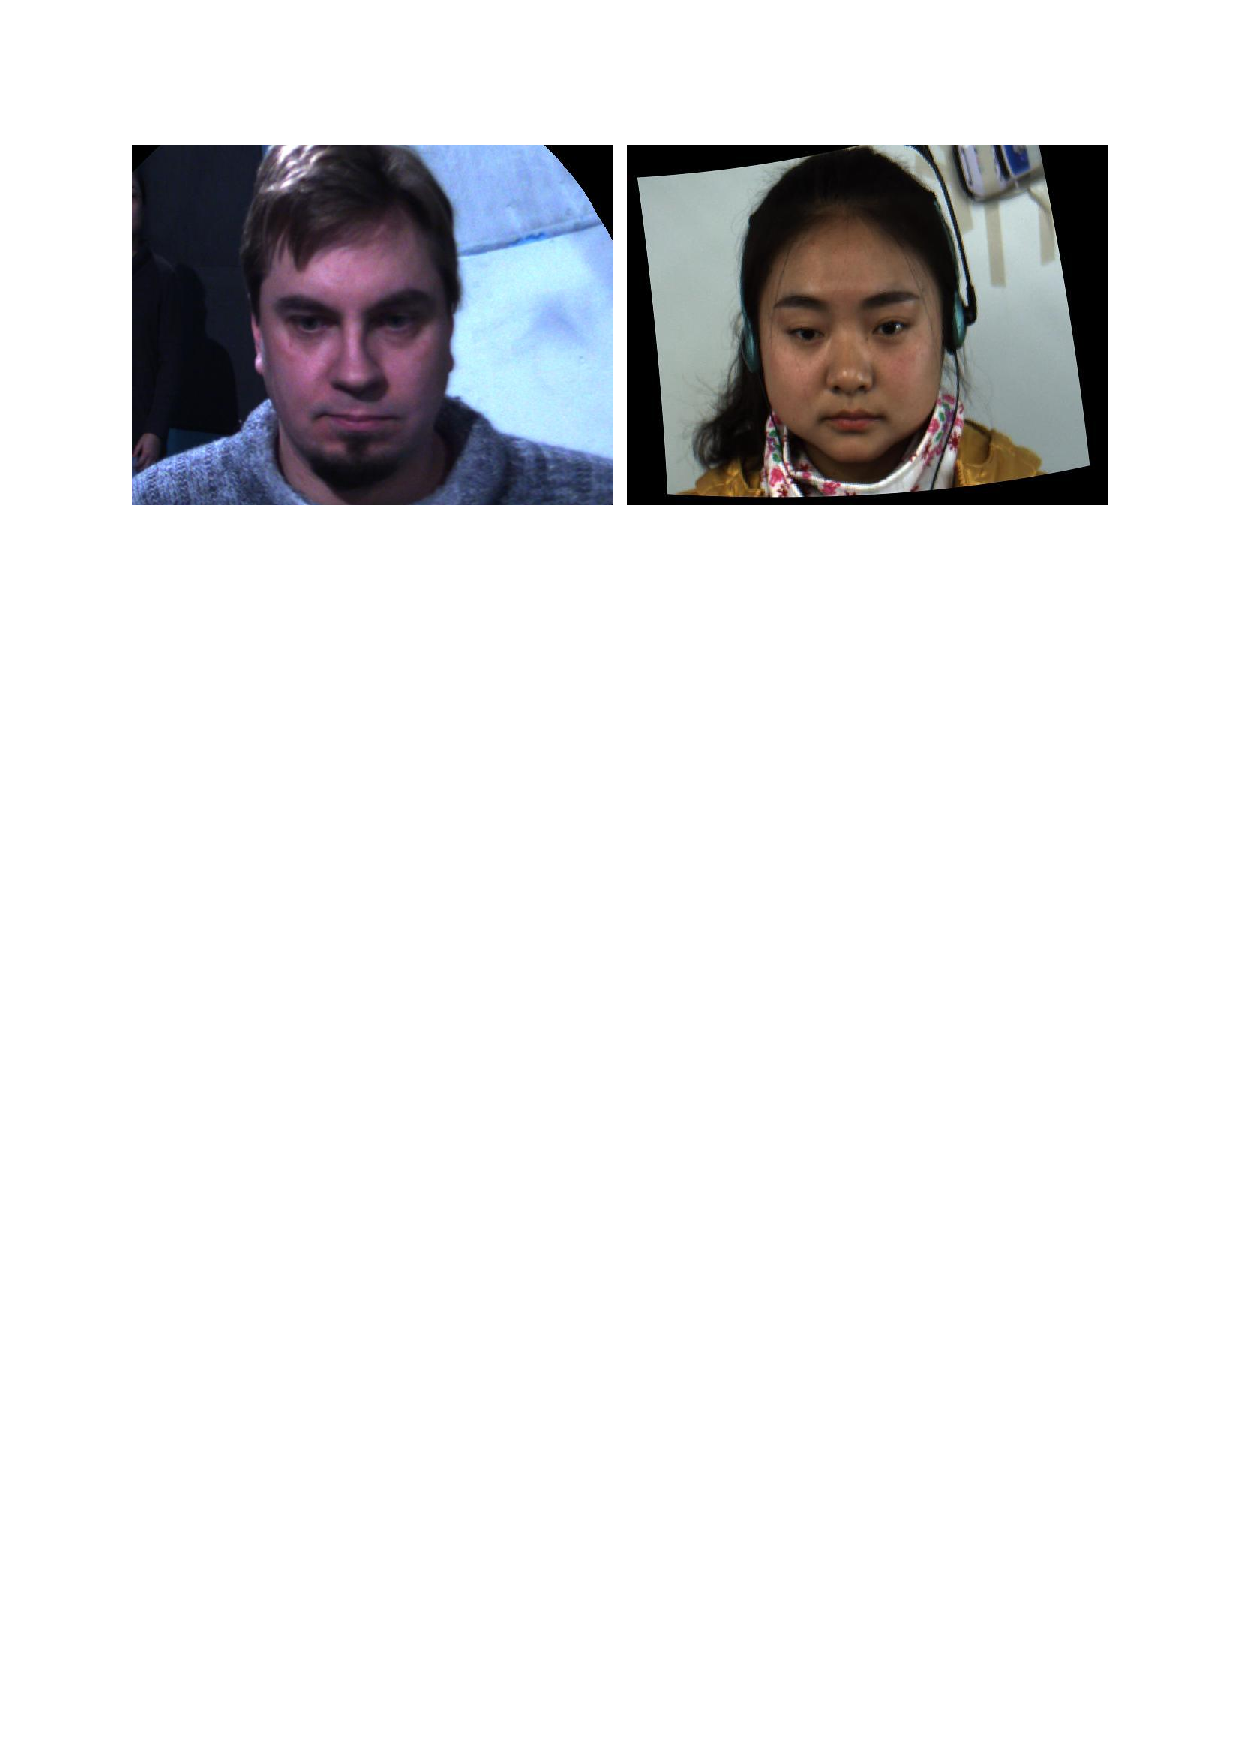
\includegraphics[width=0.65\textwidth]{3LR2}
\caption{LWM算法人脸对齐后的图像}
\label{fig13}
\end{figure}

\subsection{时间插值模型}

微表情视频有不同的长度,从4帧到50帧(如果用100帧/秒的相机拍摄)。为了解决视频片段长度不同的问题,Li等人利用TIM算法将序列的所有帧映射到曲线上,对新合成的人脸图像进行固定间隔采样,最终得到相同的预定义序列长度。实验结果表明,该算法提高了识别精度。图~\ref{fig14}显示了TIM的映射过程\citep{zhou2011towards}。

\begin{figure}[!htbp]
\centering
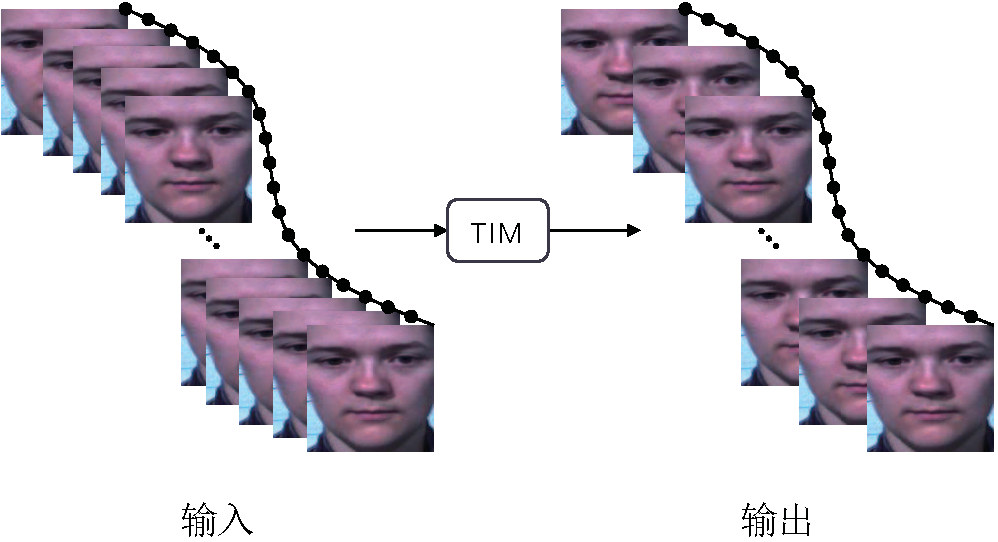
\includegraphics[width=0.65\textwidth]{LR2}
\caption{输入为原始图像序列,输出为TIM算法插值后图像序列}
\label{fig14}
\end{figure}

对由重建出的高分辨率图像组成的图像序列应用TIM算法统一帧数。具体操作为:将重建的图像序列映射到一条非线性曲线上$\mathcal{F}^{n}:\left [ 1/n,1 \right ]\rightarrow \mathbb{R}^{n-1}$ ,
\begin{equation}
    \label{eq4}
    \mathcal{F}^{n}(t)=\begin{bmatrix}f_{1}^{n}(t)\\ f_{2}^{n}(t)\\ \vdots \\ f_{n-1}^{n}(t)\end{bmatrix}
\end{equation}
其中$f_{k}^{n}(t)=sin(\pi kt+\pi (n-k)/n),\quad t\in \left [ 1/n,1 \right ]$ ,$n$为视频段中帧数(图像序列个数),根据实验需求等间距采样,获得统一帧数。

Another special challenge of ME recognition is the short duration. For example, the shortest clip in SMIC lasts for 3/25 seconds, which has only three frames (at 25 fps). Such short sequences strictly limited the application of many spatial-temporal feature descriptors, e.g., for the LBP-TOP feature feasible radius along the time dimension can only be r = 1. Besides, there are also considerable big length variations between ME clips. This also poses a challenge for some features that are sensitive to the frame number.
另一个对自我认知的特殊挑战是持续时间短。例如,SMIC中最短的剪辑持续3/25秒,只有3帧(25 fps)。这样的短序列严格限制了许多时空特征描述符的应用,例如LBP-TOP特征沿时间维的可行半径只能为r = 1。除此之外,ME夹之间也有相当大的长度变化。这也对一些对帧号敏感的特性提出了挑战。

In Zhou et al. (2011), a temporal interpolation model (TIM) was proposed, which in the original paper was for the purpose of lip-reading. We employ the TIM method in our ME recognition framework to counter for the problem related with ME durations and frame number variances.
Zhou等人提出了一种时间插值模型(TIM),该模型在原论文中是用于唇读的。我们在ME识别框架中使用TIM方法来解决与ME持续时间和帧数方差相关的问题。

The TIM method relies on a path graph to characterize the structure of a sequence of frames. A sequence-specific mapping is learned to connect frames in the sequence and a curve embedded in the path graph so that the sequence can be projected onto the latter. The curve, which is a continuous and deterministic function of a single variable t in the range of [0,1], governs the temporal relations between the frames. Unseen frames occurring in the continuous process of an ME are also characterized by the curve. Therefore a sequence of frames after interpolation can be generated by controlling the variable t at different time points accordingly.
TIM方法依赖于一个路径图来描述帧序列的结构。学习序列特定映射,将序列中的帧与路径图中嵌入的曲线连接起来,从而将序列投影到路径图中。曲线是[0,1]区间内单个变量t的连续确定性函数,控制着帧间的时间关系。在ME的连续过程中出现的不可见的帧也可以用曲线来表征。因此,通过控制变量t在不同时间点的变化,可以生成插值后的帧序列。

With the TIM method we are able to change the frame sequences into any arbitrary length, for either down-sampling or up-sampling. In the current framework, the TIM method was used to interpolate all ME clips (of one dataset) into one fixed length, e.g., of 10, 20, or 40 frames. By unifying the clips length, we can solve both the problem of short duration, and the problem of varied sequence lengths. The purpose of the current step is for 1) allowing more options when selecting feature parameters, and 2) achieving more stable performance with spatial-temporal feature descriptors. The problem of how to select the most suitable length for TIM interpolation is explored and discussed in the Section 2.4.2.
使用TIM方法,我们可以将帧序列改变为任意长度,无论是向下采样还是向上采样。在目前的框架中,TIM方法被用来将所有的ME剪辑(一个数据集)插入到一个固定的长度,例如,10帧、20帧或40帧。通过统一剪辑长度,既可以解决短持续时间的问题,也可以解决序列长度变化的问题。当前步骤的目的是1)在选择特征参数时允许更多的选项,2)利用时空特征描述符实现更稳定的性能。如何选择最合适的TIM插值长度的问题在2.4.2节中进行了探讨和讨论。

\section{超分辨重建过程}

低分辨率图像和高分辨率图像在质量和分辨率上都是不同的。高分辨率图像序列的微表情识别方法不能直接应用于低分辨率图像序列。在2.1节中,我们介绍了从高分辨率图像生成低分辨率图像的过程。

为了重建高分辨率图像,论文\citepns{shi2018hallucinating}提出了一种新的人脸幻觉算法。将基于块的正则化项与基于像素的正则化项相结合,对目标函数进行约束。重构后的高分辨率图像$\boldsymbol{H}$可以通过最小化以下目标函数得到:
\begin{equation}
 \label{eq4}
 \begin{split}
    f\left ( \boldsymbol{H} \right )= \left \| \boldsymbol{L}-\boldsymbol{DBH} \right \|{_{2}^{2}}+\alpha \boldsymbol{F}_{patch}+\eta \boldsymbol{F}_{pixel}+\lambda \boldsymbol{F}_{penalty}
 \end{split}
\end{equation}
其中右侧第一项为重建误差,后三项分别是基于块的正则项、基于像素的正则项以及惩罚项。图~\ref{fig15}展现了重建工作的具体流程。具体将在下文详细介绍。

\begin{figure}[!htbp]
\centering
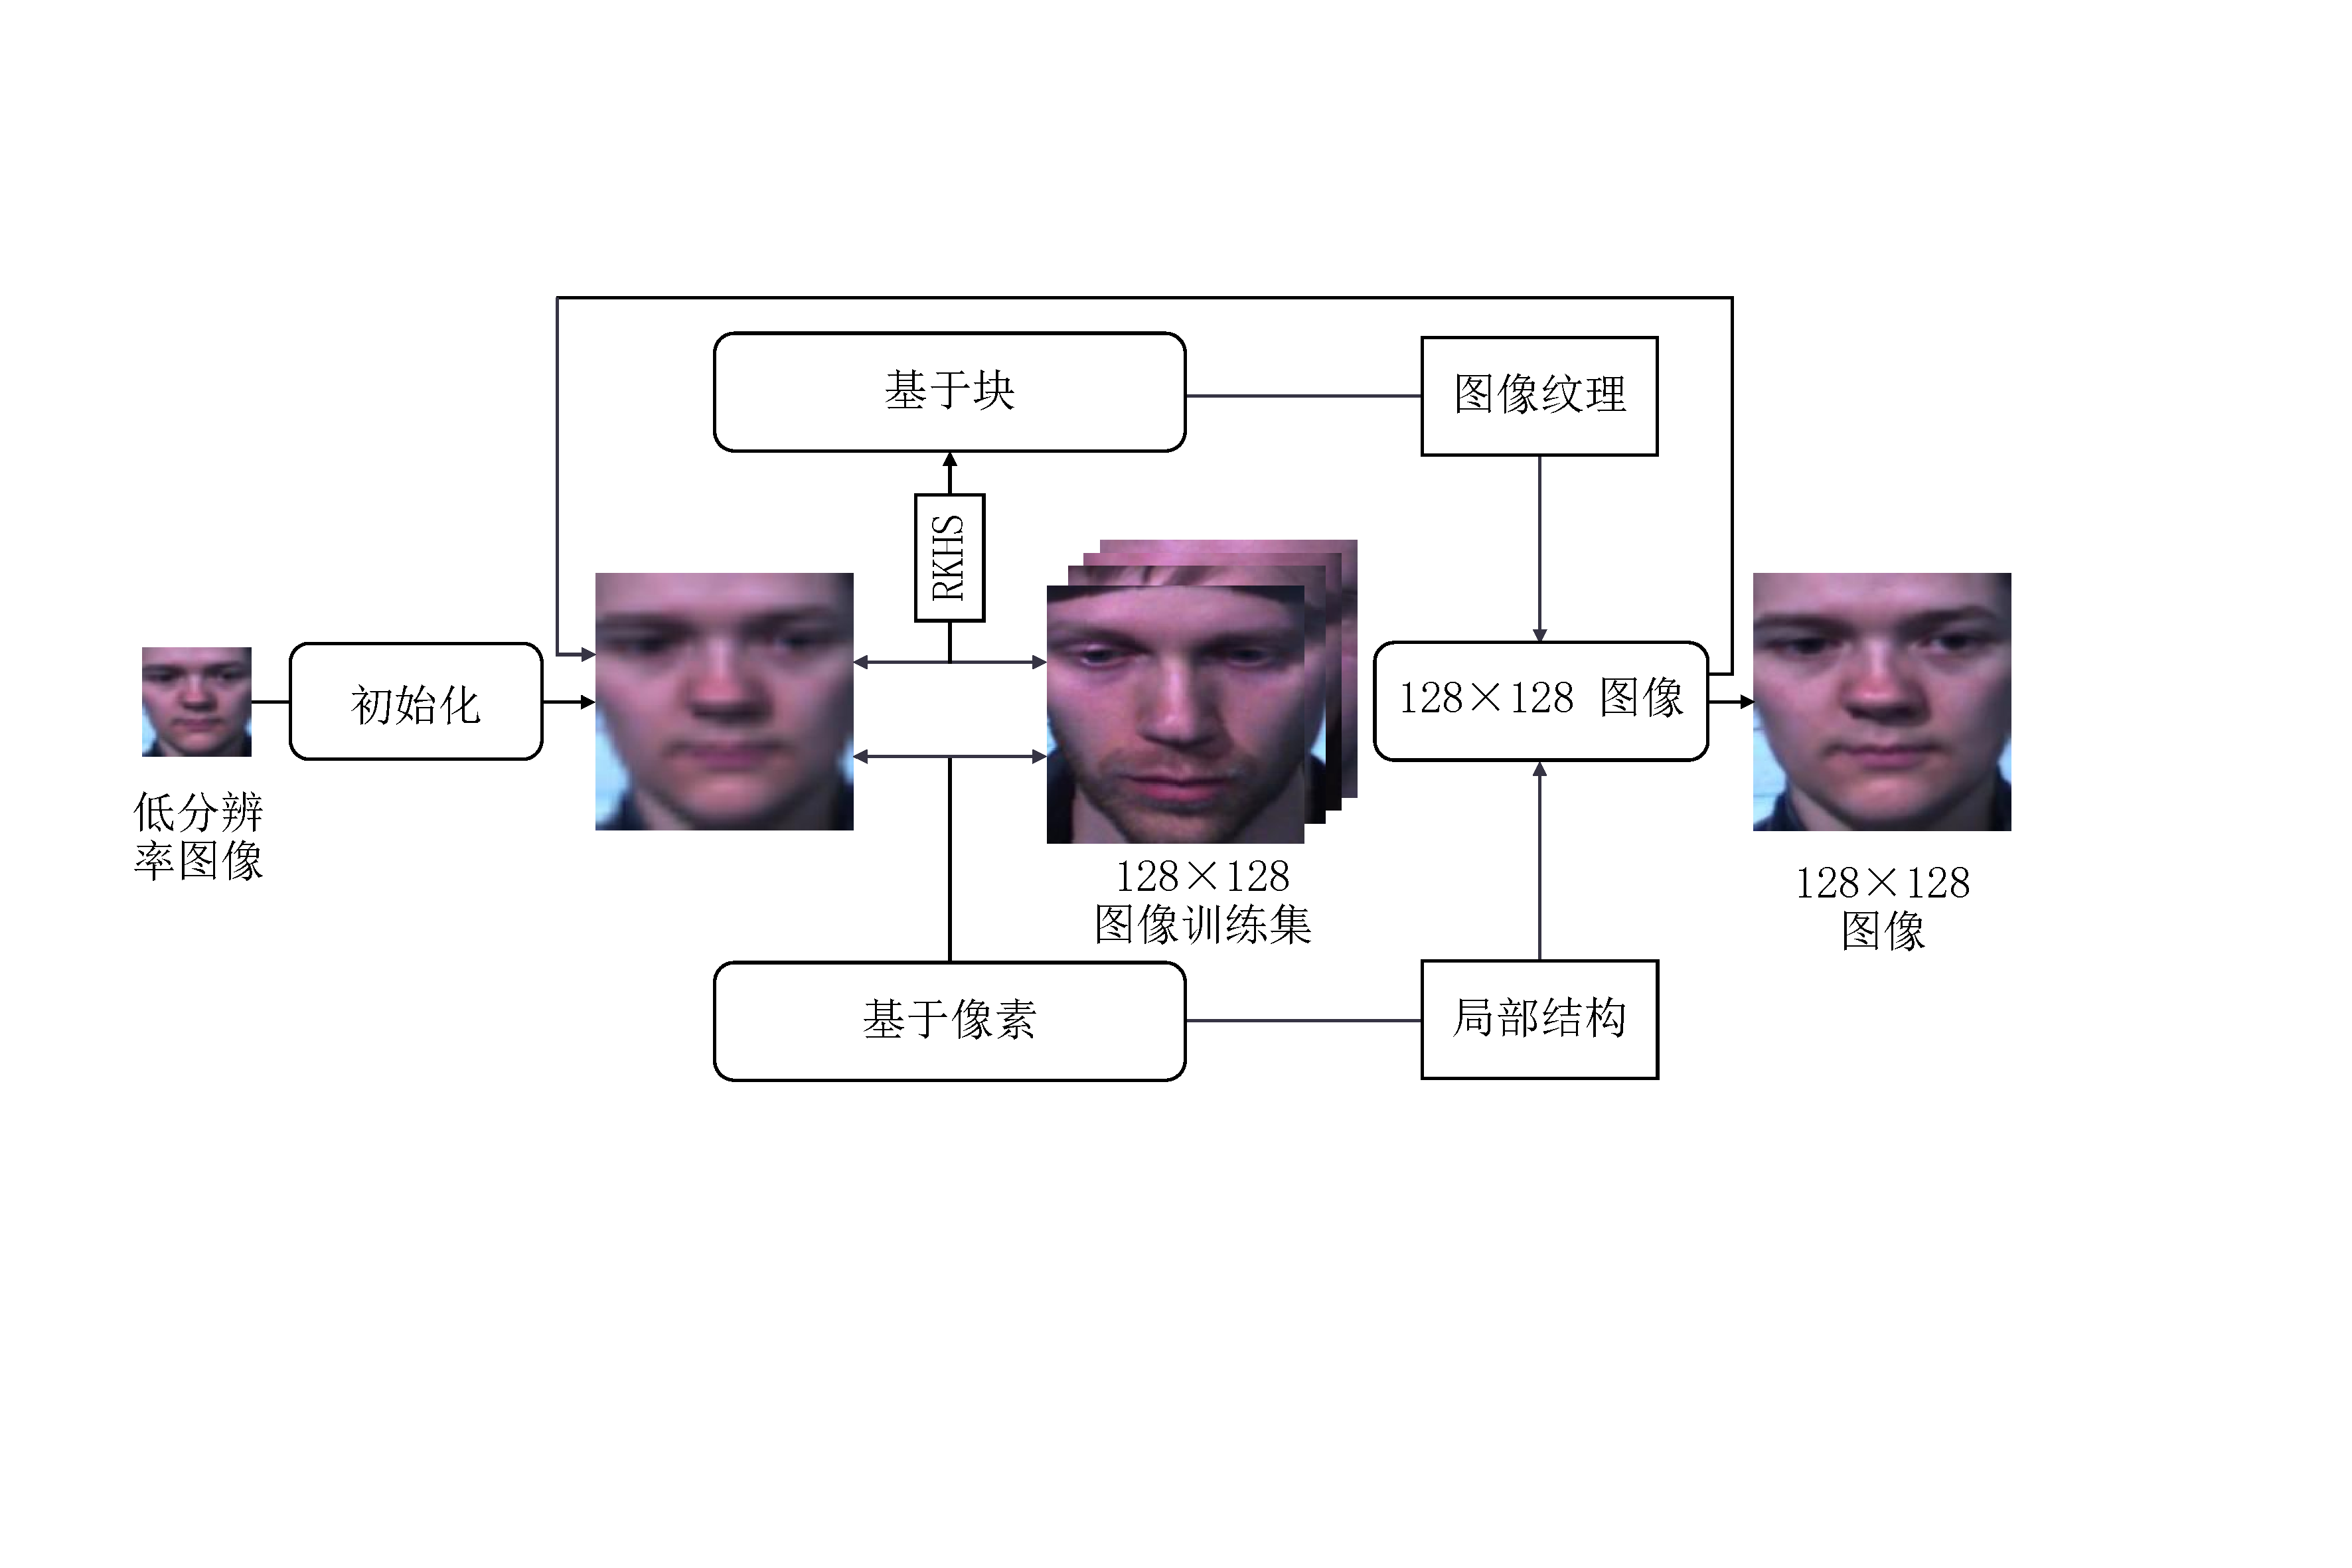
\includegraphics[width=0.75\textwidth]{LR3}
\caption{超分辨重建过程}
\label{fig15}
\end{figure}

\subsection{基于的块方法}

将分割后的图像$\boldsymbol{L}$(低分辨率图像)应用三线性插值法调整为与训练样本图像$\boldsymbol{H}$(高分辨率图像,来自公开的高分辨率图像集)大小相等的尺寸,将此图命为$\boldsymbol{H^{(0)}}$(超分辨重建过程的初始图像),对图像分块处理(如分块数为$8\times8$),如图7所示,最小化代价函数:
\begin{equation}
 \label{eq5}
 \begin{split}
   \boldsymbol{J_{\tau }(\omega _{\tau },H^{(k)})} & =\left \{ \left \| \boldsymbol{\phi (R_{\tau }H^{k})}-\boldsymbol{\phi (H_{\tau })\omega _{\tau }} \right \| _{2}^{2}+\boldsymbol{\lambda} \left \| \boldsymbol{d_{\tau }}\bigotimes \boldsymbol{\omega _{\tau }} \right \|_{2}^{2}\right \} \\
   \boldsymbol{s.t. 1^{T}\omega _{\tau }}= 1 & ,2,\cdots ,M
 \end{split}
\end{equation}
估算结合系数$\boldsymbol{\omega _{\tau }}$ ,将其初始结合系数命名为$\boldsymbol{\omega_{\tau }^{0}}$,此时$\boldsymbol{H^{(k)}}$ 已知,即$\boldsymbol{H^{(0)}}$ ,其中$\boldsymbol{\tau}$为图像中图像块的位置,$\boldsymbol{R_{\tau }}$为提取所有图像集位置$\tau$的图像块的矩阵, $\boldsymbol{H_{\tau }}=\left [ h_{\tau }^{1},\cdots ,h_{\tau }^{N} \right ]$为高分辨率图像位置$\boldsymbol{\tau}$处图像块集($N$为训练样本的数量,即高分辨率图像集的数量),$\boldsymbol{\phi (\cdot )}$ 为从原始空间到无限维再生核希尔 伯特空间(Reproducing Kernel Hilbert Space, RKHS)的映射,$\boldsymbol{d_{p}}$ 描述了目标高分辨率块(重建出的块)与相应的训练样本块在核映射空间的核相似性,$\bigotimes$ 表示哈达玛积,$\boldsymbol{\lambda}$为惩罚参数,$\boldsymbol{1}$为全为1的列向量,$M$为图像的块数。

将获得的$\boldsymbol{\omega _{\tau }}$($\boldsymbol{\omega_{\tau }^{0}}$)代入公式(5),并最小化:
\begin{equation}
 \label{eq6}
 \begin{split}
   \boldsymbol{f(H)}= \left \| \boldsymbol{L^{k}}-\boldsymbol{DBH^{k}} \right \|_{2}^{2}+\boldsymbol{\eta \sum_{\tau }}\left \| \boldsymbol{x_{\tau }h^{k}}-\boldsymbol{\beta _{\tau }H_{\tau }} \right \|_{2}^{2}+ \\
   \boldsymbol{\alpha \sum_{\tau }}(\left \| \boldsymbol{\phi (R_{\tau }H^{k})}-\boldsymbol{\phi (H_{\tau })\omega _{\tau } }\right \|_{2}^{2}+ \boldsymbol{\lambda} & \left \| \boldsymbol{d_{\tau }}\bigotimes \boldsymbol{\omega _{\tau } }\right \|_{2}^{2})+\boldsymbol{\sigma MSE} \\
   \boldsymbol{s.t. \quad 1^{T}\omega _{\tau }}= 1,2,\cdots ,M \qquad \qquad \qquad \qquad \qquad \quad &
 \end{split}
\end{equation}
获得重建的高分辨率图像$\boldsymbol{H^{(k)}}$(初始结果命名为$\boldsymbol{H^{(1)}}$),其中$\boldsymbol{D}$为下采样矩阵,$\boldsymbol{B}$为模糊处理矩阵,$\boldsymbol{\beta _{\tau }}$为规范全局优化的像素间关系矩阵,$\boldsymbol{MSE}$为均方误差,$\boldsymbol{\eta }$为基于像素正则项的权重,$\boldsymbol{\alpha}$为基于块正则项的权重,$\boldsymbol{\sigma}$为均方误差的权重。

\subsection{基于像素的方法}


\section{微表情的特征提取与分类}

如图~\ref{fig10}所示,微表情识别主要分为两部分:特征提取和分类。在以往的微表达分析方法中研究人员展示了LBP-TOP及其变体作为特征描述符的优势。与传统的基于单个图像的LBP特征不同,LBP-TOP可以捕捉到空间和时间域的动态变化,这对于微表情识别是必不可少的。我们首先将整个人脸图像序列划分为几个长方体,如$ 5\times5\times1 $,$ 8\times8\times2 $等,其中前两个参数决定了空间域中的块数,最后一个参数是时间方向上的段数。每个长方体都可以看作一个新的单位。LBP特征提取自新单元中三个不同的正交平面(XY、XT、YT)。我们遍历所有长方体,得到图像序列的LBP-TOP特征,然后将每个长方体的LBP-TOP特征串联起来。如图5所示。

在分类部分,我们使用线性支持向量机(LSVM)作为分类器\citep{chang2011libsvm}。为了进行公平的比较,我们在实验中采用了一主体退出协议。根据数据集发布方提供的微表情表签,我们将来自SMIC的样本分为三类(positive, negative, surprise),来自CASME II的样本分为五类(happiness, surprise, repression,disgust, and other)。

As mentioned in the literature review section, spatial-temporal descriptors are the major stream in most of ME analysis studies. Three kinds of spatial-temporal features are considered here in the proposed ME recognition framework. Details of each feature are briefly described below, and the comparison of their performance will be discussed with experimental results in Section 2.4.2.
如文献综述部分所述,时空描述符是ME分析研究的主流。本文提出的ME识别框架考虑了三种时空特征。下面将简要描述每个特性的细节,并将在2.4.2节中与实验结果进行比较。

\subsection{LBP-TOP特征提取}

The first feature is the local binary pattern on three orthogonal planes (LBP-TOP), proposed by Zhao \& Pietikäinen (2007). LBP-TOP is an extension of the original LBP for dynamic texture analysis in spatial-temporal domain. According to our literature review, LBP-TOP and its variants are the most frequently used features in current ME recognition studies.
第一个特征是三个正交平面上的局部二元模式(LBP-TOP),由Zhao \& Pietikainen(2007)提出。LBP- top是原LBP的扩展,用于时空域的动态纹理分析。根据我们的文献综述,LBP-TOP及其变体是目前ME识别研究中最常用的特征。

A video sequence can be thought as a cuboid of pixels on X, Y and T dimension. Traditional LBP code can be extracted from either XY, XT or YT plane, as shown in Figure 5(a). To summarize spatial-temporal attributes of the 3D cuboid, the three LBP histograms from each plane are concatenated into a big histogram as the final LBP-TOP feature vector, as illustrated in Figure 5(b).
视频序列可以看作是X、Y和T维上像素的长方体。传统的LBP代码可以从XY、XT或YT平面中提取,如图5(a)所示。为了总结三维长方体的时空属性,将每个平面的三个LBP直方图拼接成一个大直方图作为最终的LBP- top特征向量,如图5(b)所示。


\subsection{LSVM}

Although the selection of classifier is also important, it is not considered as the main target for the current research. To keep it well-controlled and put more focus on previous steps of the framework, in all the following ME recognition experiments, we use a linear SVM (Chang \& Lin 2011) as the classifier and use the leave-one-subject-out protocol for validation. For the tests on SMIC, ME samples are classified into three categories; for the tests on CASMEII, ME samples are classified into five categories.
虽然分类器的选择也很重要,但它并不是目前研究的主要目标。为了保持良好的控制,并将更多的注意力放在框架的前几个步骤上,在接下来的ME识别实验中,我们使用了线性SVM (Chang \&amp;Lin 2011)作为分类器,使用leave-one-subject-out协议进行验证。对于中芯国际的测试,ME样本分为三类;对于CASMEII的测试,ME样本分为五类。

支持向量机(Support Vector Machine, SVM)是曾经打败神经网络的分类方法,从90年代后期开始在很多领域均有举足轻重的应用,近年来,由于深度学习的兴起,SVM的风光开始衰退,但是其仍然不失为一种经典的分类方法。SVM最初由 Vladimir N. Vapnik 和 Alexey Ya. Chervonenkis于1963年提出,之后经过一系列改进,现今普遍使用的版本由Corinna Cortes 和 Vapnik于1993年提出,并在1995年发表。深度学习兴起之前,SVM被认为是机器学习近几十年来最成功、表现最好的方法。

本文讨论线性可分的支持向量机,详细推导其最大间隔和对偶问题的原理。简单起见,以二分类为例,如下图,设训练集为D={(x1,y1),...,(xn,yn)}D={(x1,y1),...,(xn,yn)},蓝色圆点为一类,红色方块为另一类,分类的目标是寻找一个超平面,将两类数据分开。在二维平面中,分类超平面就是一条直线,从图中可以看出,能将训练样本分开的超平面有很多可能(图中绿色虚线),超平面除了要将训练集中的数据分开,还要有较好的泛化性能,需要把测试集中的数据也划分开。从直观上看,绿色实线是比较好的一个划分,因为该直线距离两类数据点均较远,对于数据局部扰动的容忍性较好,能够以较大的置信度将数据进行分类。


\section{实验设置及分析}

The proposed framework was tested on two databases of SMIC and CASMEII. In order to explore the effect of each individual step of the framework, four sub-experiments were carried out each for a different purpose. The sub-experiments and their results are described in below.
该框架在中芯国际和CASMEII两个数据库上进行了测试。为了探究框架中每个单独步骤的效果,我们针对不同的目的分别进行了四个子实验。子实验及其结果如下所述。

Effect of TIM Interpolation
TIM插值的效果

In the first sub-experiment we would like to evaluate how the interpolation process will affect the performance of the framework. We also hope to find a suitable sequence length (or length range) for the interpolation process that would be efficient for the ME recognition task.
在第一个子实验中,我们想要评估插值过程将如何影响框架的性能。我们也希望找到一个合适的序列长度(或长度范围)的插值过程,将是有效的ME识别任务。

To avoid the impact from other factors and focus on the TIM process, we skip the motion magnification step and use only LBP-TOP (with fixed parameters of 8 8 1 blocks, r = 2, p = 8) as the feature descriptor. We choose eight interpolation lengths (10, 20, ..., 80) for the TIM step, and evaluate the framework on SMIC-HS, SMIC-VIS and SMIC-NIR datasets. The average sequence length of the original ME clips is 33.7 frames for SMIC-HS and 9.66 frames for SMIC-VIS and SMIC-NIR.
原始ME片段的平均序列长度为SMIC-HS为33.7帧,SMIC-VIS为9.66帧,SMIC-NIR为9.66帧。为了避免其他因素的影响,将重点放在TIM过程上,我们跳过了运动放大的步骤,只使用LBP-TOP(参数固定为881个block, r = 2, p = 8)作为特征描述符。我们选择8个插值长度(10,20,…)对于TIM步骤,对SMIC-HS、SMIC-VIS和SMIC-NIR数据集的框架进行评估。


Test results are shown in Figure 6. The results can be summarized in two aspects. First, interpolation to 10 frames (TIM10 for short) leads to significantly better perfor mance than without the TIM process. Compared to the original sequences, TIM10 barely changed the average sequence lengths for SMIC-VIS and SMIC-NIR, and it was a down-sampling process for SMIC-HS. Thus we think the improved performance was caused by the unifying of the sequences length. Secondly, if we compare the result of TIM10 to those of longer TIM sequences, it shows that longer interpolated sequences do not lead to better performance. One possible explanation for this result might be that, the time-dimension changes are diluted if the ME clips are interpolated into much longer sequences. According to the two findings, it appears that TIM of 10 frames is the best option for the current framework. In all the following experiments, TIM10 is applied in the framework as default if not otherwise specified.
测试结果如图6所示。研究结果可以归纳为两个方面。首先,插值到10帧(简称TIM10)比不使用TIM过程的perfor mance要好得多。与原始序列相比,TIM10几乎没有改变SMIC-VIS和SMIC-NIR的平均序列长度,是SMIC-HS的下采样过程。因此,我们认为序列长度的统一导致了性能的提高。其次,如果我们将TIM10的结果与较长的TIM序列的结果进行比较,就会发现较长的插值序列并不会带来更好的性能。对这个结果的一种可能的解释是,如果ME剪辑被插值成更长的序列,时间维度的变化就会被稀释。根据这两个发现,对于目前的框架来说,TIM of 10 frames似乎是最好的选择。在接下来的所有实验中,如果没有另外指定,TIM10将作为默认值应用于框架中。

Comparison of features
特性的比较

The purpose of the second sub-experiment is to compare the performance of three features. Five combinations of histograms on three orthogonal planes of each feature are evaluated separately.
第二个子实验的目的是比较三个特征的性能。在每个特征的三个正交平面上分别计算五种直方图组合。

After face alignment, TIM10 were applied to interpolate all sequences into 10 frames. The motion magnification step was temporally skipped for later discussion. Three kinds of features were extracted from evenly divided blocks of sequences with varied parameters. For the LBP feature, we vary the radius r, neighbour points p and the number of divided blocks; for the HOG and HIGO features, we fixed the number of bins as b = 8 and vary the number of divided blocks. Tests were carried out on three datasets of SMIC and CASMEII, and the results are listed in Table 5. Note that results of the five combinations of three orthogonal planes of each feature are listed separately. For each combination of feature (one cell in the table), only the best result (with corresponding parameters) achieved among all parameter combinations is listed.
人脸对齐后,应用TIM10对所有序列进行10帧插值。在后面的讨论中暂时跳过了运动放大步骤。从不同参数序列的均匀分割块中提取三种特征。对于LBP特征,我们改变半径r,邻点p和划分块数;对于HOG和HIGO特性,我们将桶的数量固定为b = 8,并改变划分块的数量。对SMIC和CASMEII的三个数据集进行了测试,结果如表5所示。注意,每个特征的三个正交平面的五个组合的结果被单独列出。对于每个特征组合(表中的一个单元格),只列出所有参数组合中获得的最佳结果(具有相应的参数)。

Two phenomenons can be found from the result table. First, the TOP combination (three orthogonal planes) doesn t always lead to the best performance, especially for the HIGO feature. In many cases better results can be achieved using only XOT, YOT or XYOT plan features, and it is true for all four datasets. On the other hand the XY plane feature always get the lowest performance than other plane combinations. The results indicate that dynamic changes along T dimension carry the most important information for ME recognition, while the XY plane features carries more about facial appearance information which maybe redundant for the ME recognition task. Similar findings were also reported in Davison et al. (2014). Secondly, comparing the three kinds of features, gradient-based features HOG and HIGO outperform LBP on three out of the four test datasets (except SMIC-NIR). HIGO seems to perform slightly better than HOG, and the highest performance obtained on SMIC is 76.06\% using HIGO-XOT. One possible explanation is that the HIGO feature is not affected by local gradient magnitude, which might vary due to the diversity of muscle movement speeds among ME clips. Results on the NIR data shows another trend. Skin textures recorded by an NIR camera are different from that of visible color videos. For the SMIC-NIR dataset, the LBP feature performed better than the other two features, which is consistent with previous results in Zhao et al. (2011).
从结果表中可以发现两个现象。首先,最上面的组合(三个正交平面)并不总是带来最好的性能,特别是对于HIGO特性。在许多情况下,仅使用XOT、YOT或XYOT计划特性就可以获得更好的结果,对于所有四个数据集都是如此。另一方面,XY平面特征总是比其他平面组合得到最低的性能。结果表明,T维上的动态变化是ME识别中最重要的信息,而XY平面特征所携带的面部特征信息更多,这可能是ME识别任务中多余的信息。Davison et al.(2014)也报道了类似的发现。其次,比较这三种特征,基于梯度的特征HOG和HIGO在四个测试数据集中的三个(SMIC-NIR除外)上优于LBP。HIGO的性能似乎略优于HOG,在SMIC上使用HIGO- xot获得的最高性能为76.06\%。一种可能的解释是HIGO特征不受局部梯度大小的影响,局部梯度大小可能由于ME片段中肌肉运动速度的多样性而变化。近红外数据显示了另一种趋势。近红外相机记录的皮肤纹理不同于可视彩色视频。对于SMIC-NIR数据集,LBP特征优于其他两个特征,这与Zhao等(2011)之前的研究结果一致。

我们现在在三个不同的自发微表达数据集上展示实验和结果,即SMIC-HS, SMIC-subHS和CASME II。实验参数的设置和结果分析将在下面的小节中讨论。

\begin{table}[!htb]
\centering
\caption{实验中使用的数据集}
\label{tab4}
\begin{tabular}{c|ccc}
\hline
 & SMIC-HS & SMIC-subHS & CASME II \\ \hline
微表情数 & 164 & 71 & 247 \\
参与者 & 16 & 8 & 26 \\
分类 & 3 & 3 & 5 \\ \hline
\end{tabular}
\end{table}

SMIC-HS和SMIC-subHS是SMIC的两个子集。SMIC-HS数据集包含来自16名参与者的164个自发微表情片段,分为三类:阳性(51个片段)、阴性(70个片段)和惊奇(43个片段)。SMIC-subHS数据集是SMIC-HS的子集,只包含最后8个参与者。前8名受试者的微表达片段数量差异较大,其中3名受试者贡献了整个组近一半的微表达样本,这可能会影响“一受试者退出”的表现,而后8名受试者的s (SMIC-subHS)片段数量分布较为均匀。SMIC-subHS数据集中,正负、惊喜片段分别为28、23、20个。同时,CASME II数据集包含26名参与者,分别属于5个不同的类别:惊讶(25个片段)、幸福(32个片段)、其他(99个片段)、厌恶(64个片段)和压抑(27个片段)。表1显示了实验中使用的数据集的摘要。面部高分辨率图像的分辨率设置为$ 128 \times 128 $的实验。$ 128 \times 128 $分辨率的图像下采样乘以2,4,8次获得低分辨率图像(如图6)。这意味着我们评估三个不同层次的低分辨率的面部图像序列(如$ 16 \times 16 $, $ 32 \times 32 $, $ 64 \times 64 $)的微识别任务。

\begin{figure}[!htb]
    \centering
    \begin{subfigure}[b]{0.35\textwidth}
      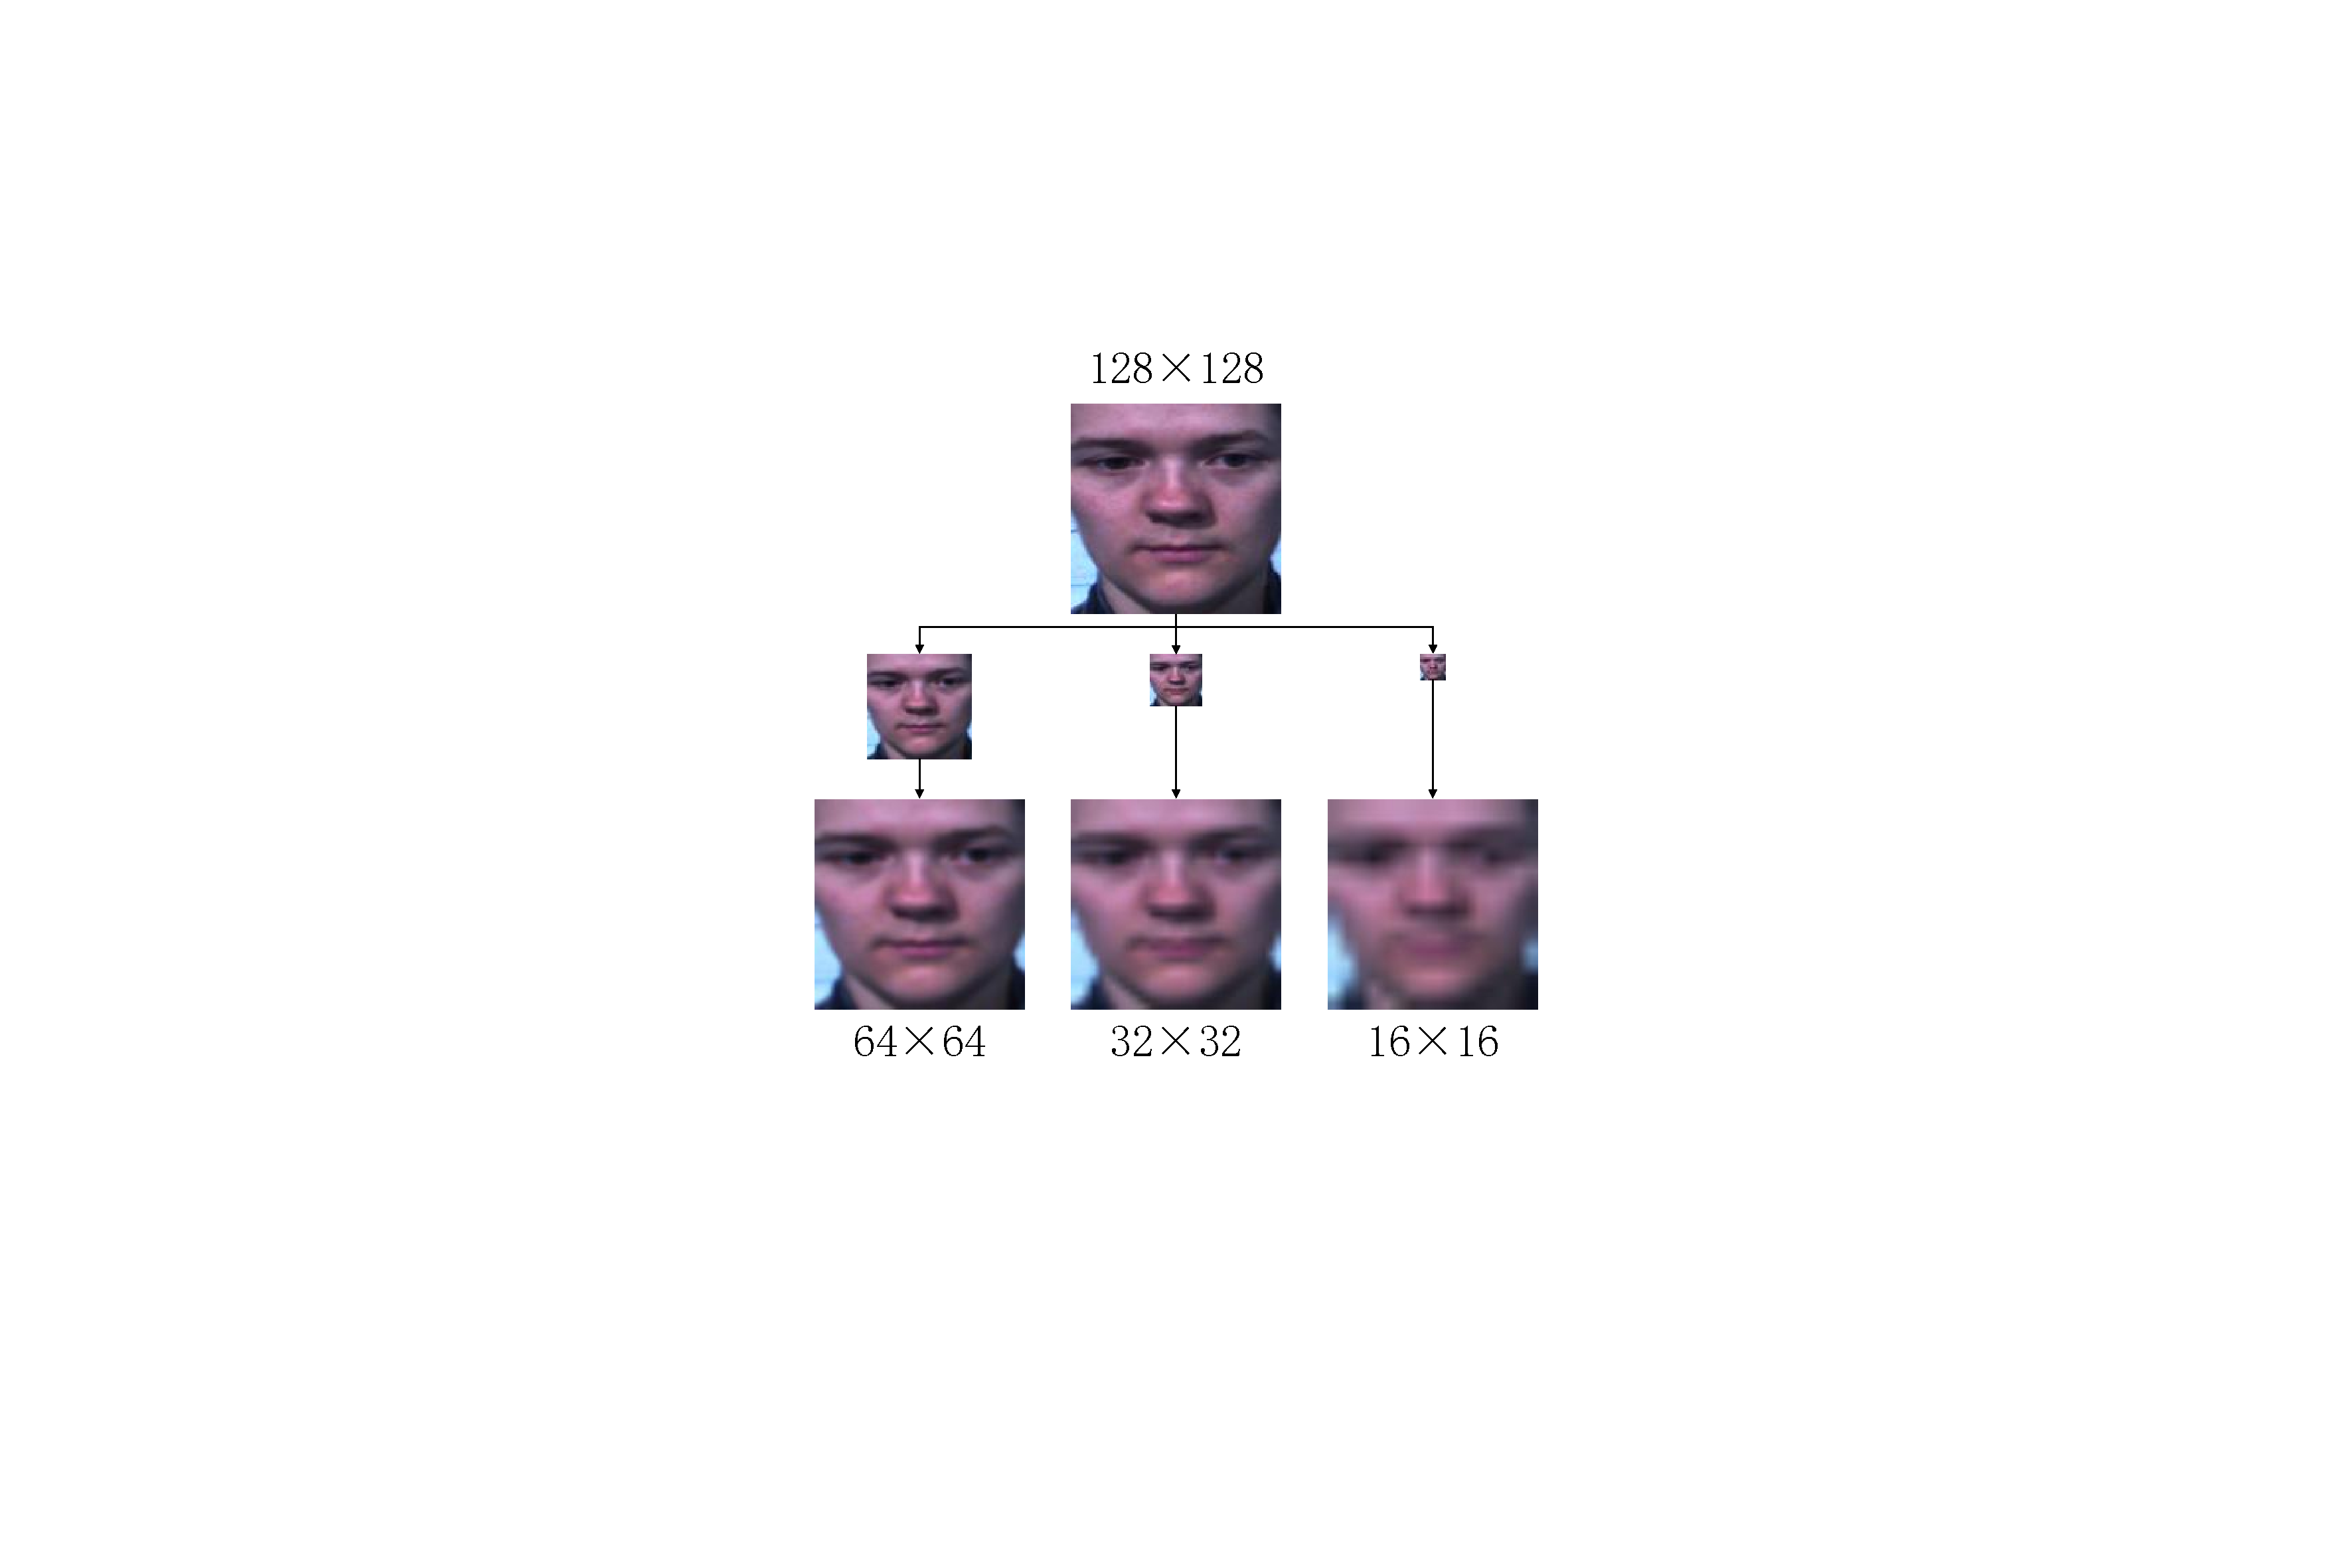
\includegraphics[width=\textwidth]{LR41}
      \caption{}
    \end{subfigure}%
    % ~ ~%add desired spacing
    \quad
    \begin{subfigure}[b]{0.35\textwidth}
      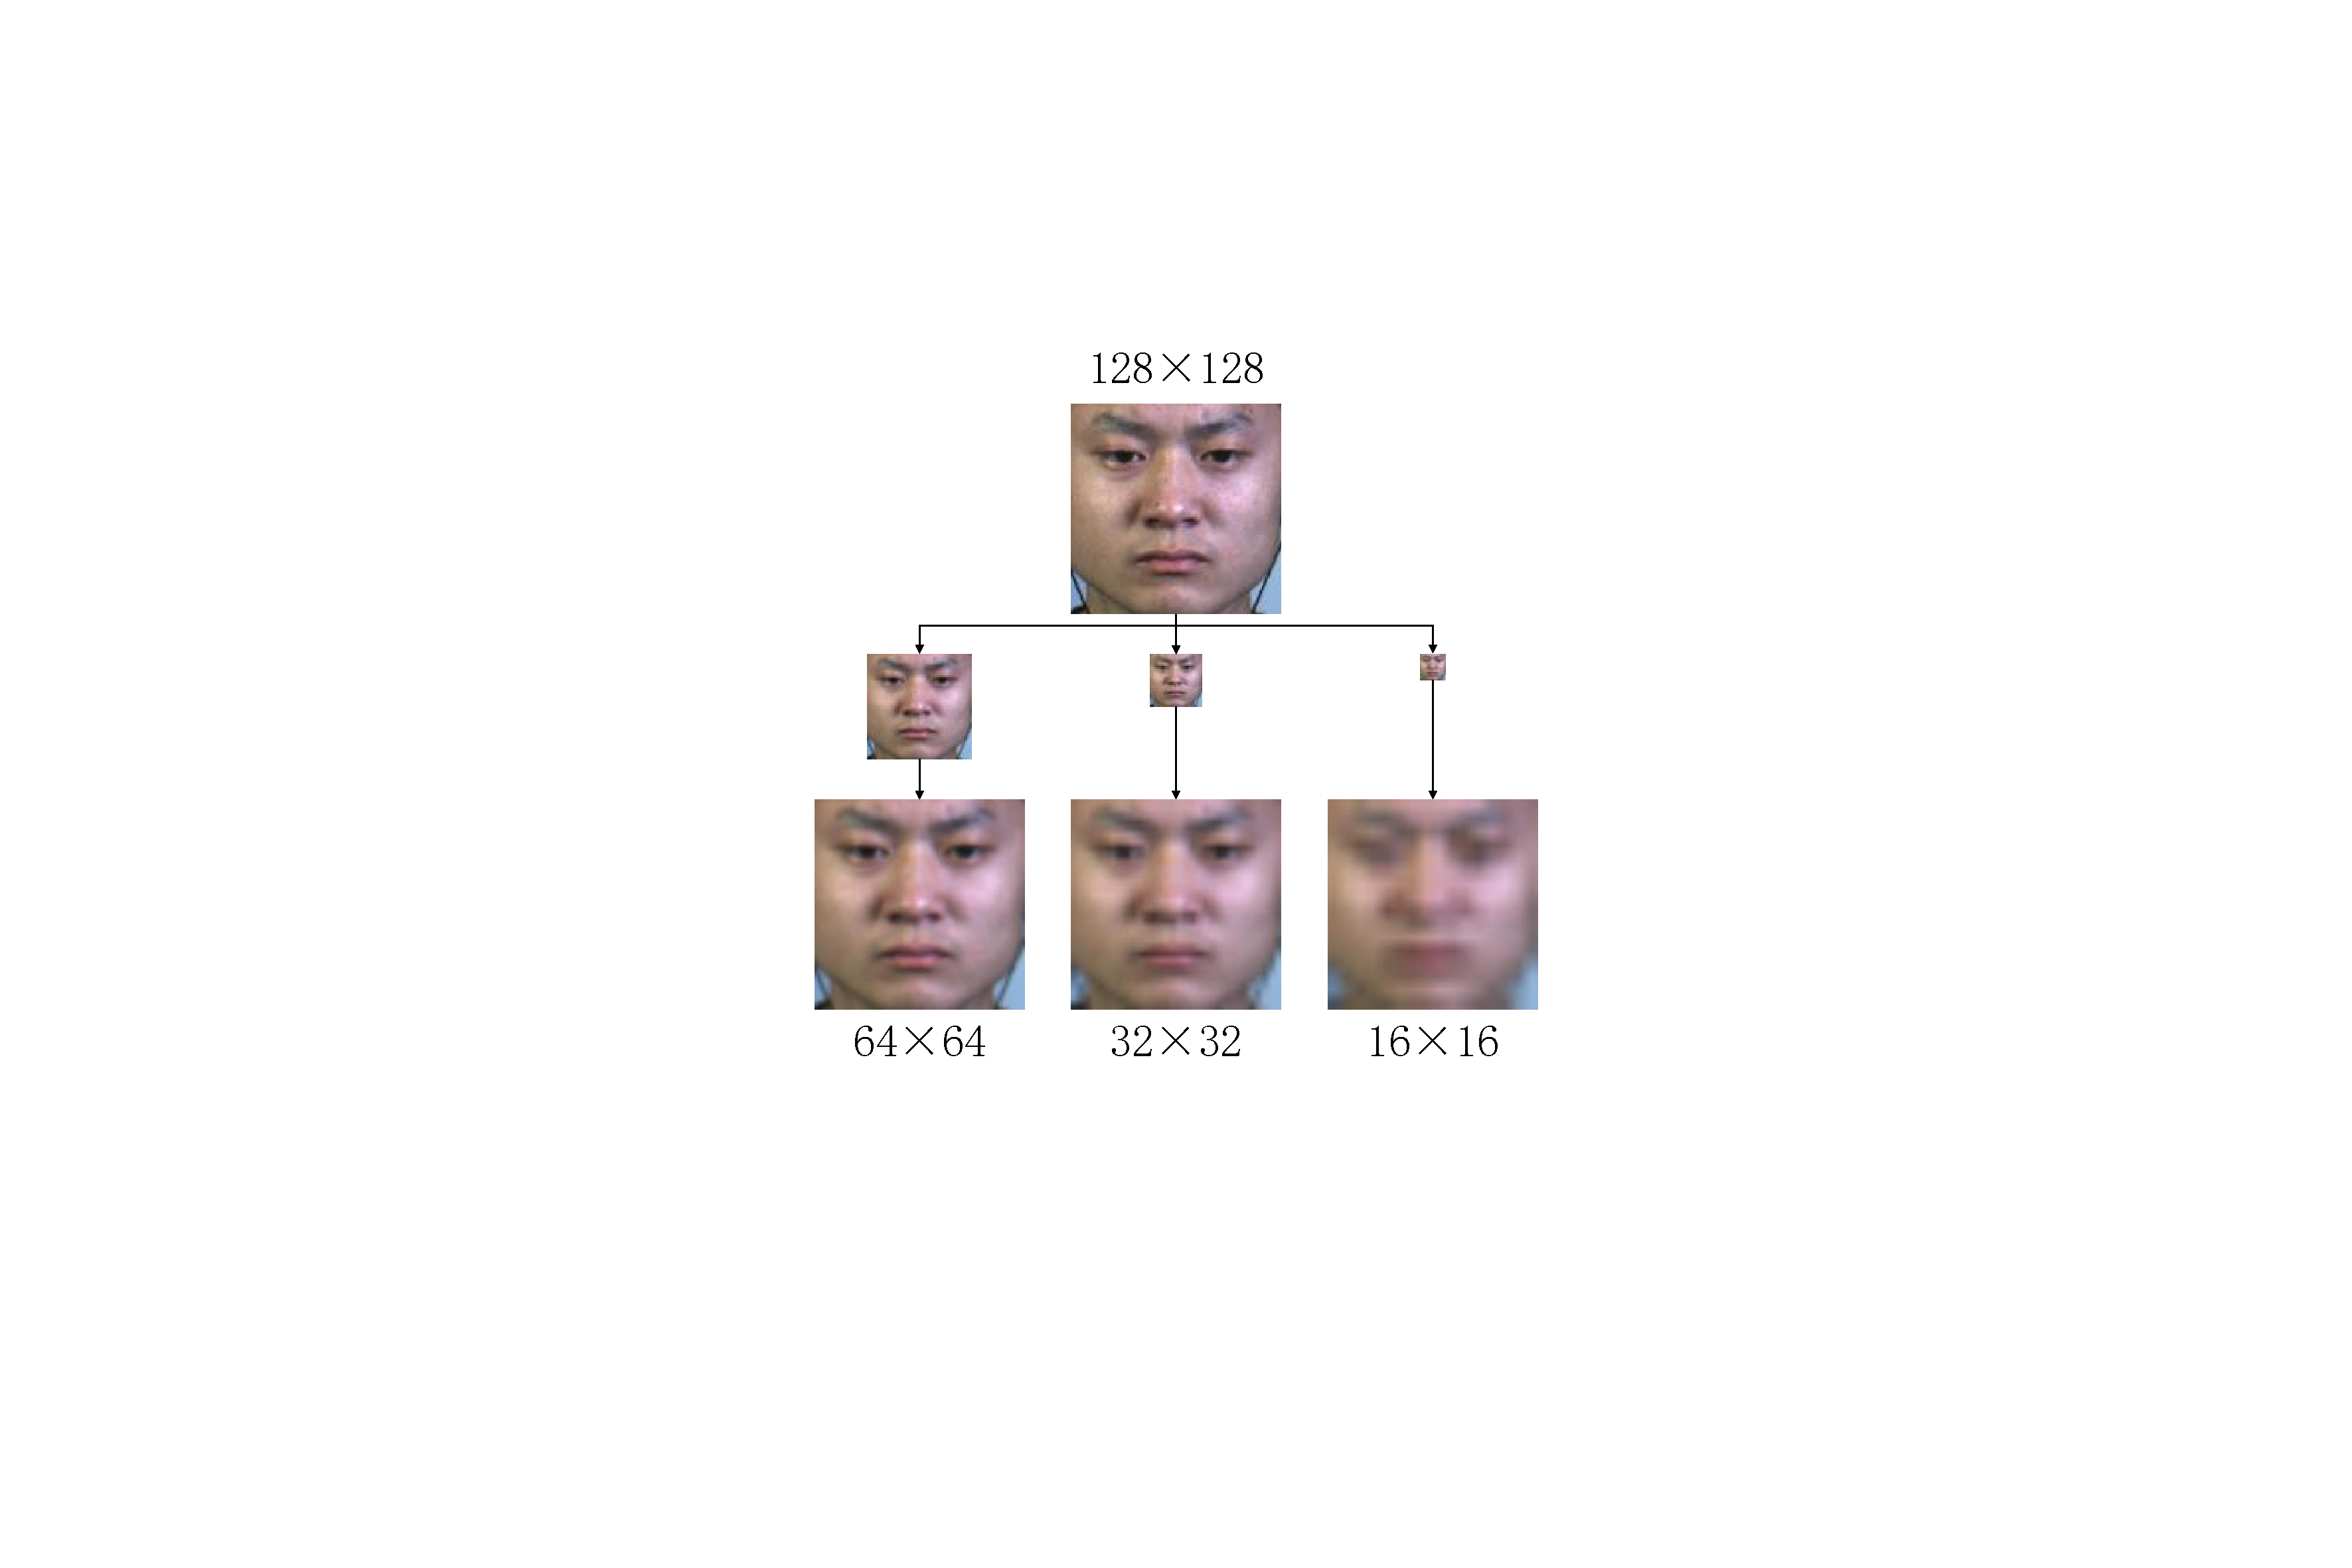
\includegraphics[width=\textwidth]{LR42}
      \caption{}
    \end{subfigure}
    \caption{低分辨率图像\\ \footnotesize \textmd{(a) SMIC-HS/SMIC-subHS数据集低分辨率图像,(b) CASME II数据集低分辨率图像}}
    \label{fig14}
\end{figure}

在本节中,利用论文\citepns{shi2018hallucinating}提出的方法将低分辨率图像重建为高分辨率图像,该方法在2.3节中进行了简要介绍。表2-3列出了不同分辨率下重建图像序列的平均峰值信噪比(PSNR)和结构相似度(SSIM)指数。在这里,我们分别使用S64、S32和S16来命名分辨率为$ 64 \times 64 $, $ 32 \times 32 $和$ 16 \times 16 $的重建图像序列。

\begin{table}[!htb]
\centering
\caption{重建图像序列的平均PSNR(dB)指标}
\label{tab5}
\scalebox{0.95}{
\begin{tabular}{c|ccc}
\hline
PSNR (dB) & $ 16 \times 16 $ & $ 32 \times 32 $ & $ 64 \times 64 $ \\ \hline
SMIC-HS & 31.25 & 37.67 & 44.30 \\
SMIC-subHS & 31.67 & 38.26 & 43.22 \\
CASME II & 31.80 & 36.49 & 37.83 \\ \hline
\end{tabular}}
\end{table}

\begin{table}[!htb]
\centering
\caption{重建图像序列的平均SSIM指标}
\label{tab6}
\scalebox{0.95}{
\begin{tabular}{c|ccc}
\hline
SSIM & $ 16 \times 16 $ & $ 32 \times 32 $ & $ 64 \times 64 $ \\ \hline
SMIC-HS & 0.9397 & 0.9775 & 0.9883 \\
SMIC-subHS & 0.8970 & 0.9346 & 0.9424 \\
CASME II & 0.9439 & 0.9761 & 0.9882 \\ \hline
\end{tabular}}
\end{table}

如表2和表3所示,重建的人脸图像序列的定量指标(PSNR/SSIM)与输入人脸图像序列的分辨率成正比。例如,在SMIC-HS数据集中,S16的PSNR指数为31.25dB,比S32低6.42dB,比S64低13.05dB。对于SSIM指数,S16达到0.9397,比S32低0.0378,比S64低0.0486。此外,图7给出了重建后的图像序列的视觉表现,也表明了与上述观点相同的结论。

\begin{figure}[!htb]
\centering
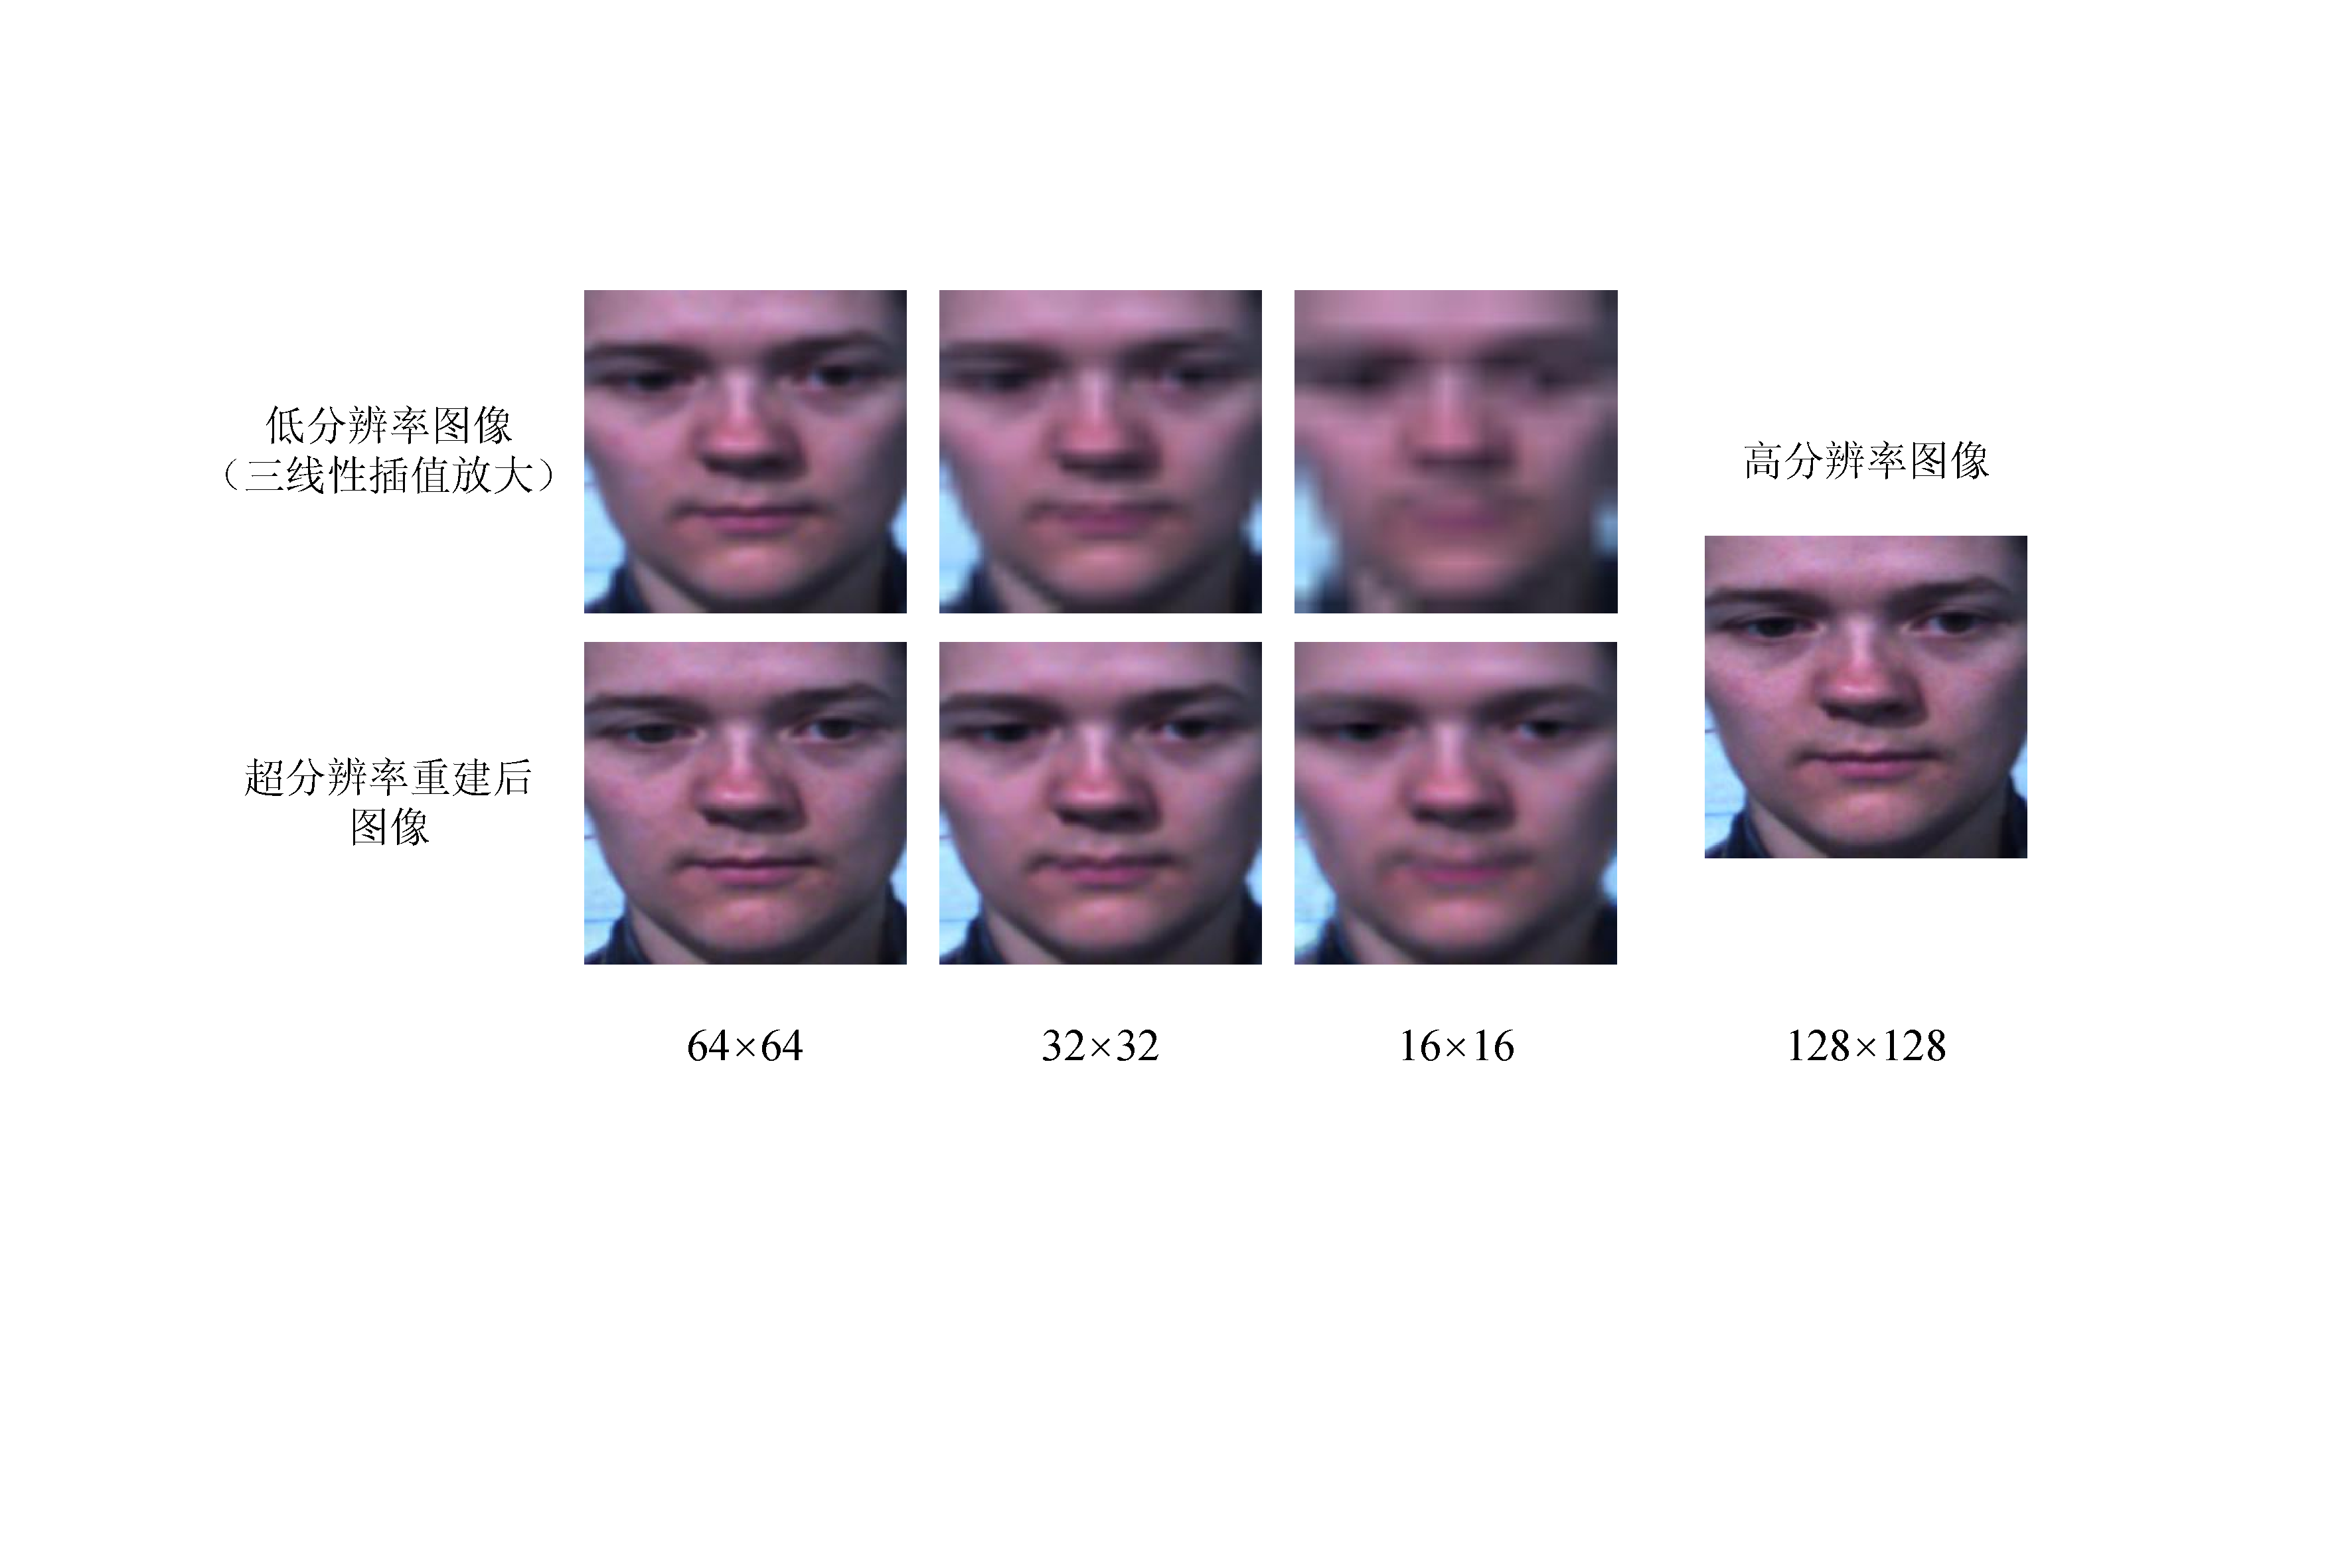
\includegraphics[width=0.75\textwidth]{LR5}
\caption{不同分辨率图像重建结果比较}
\label{fig15}
\end{figure}

为了对视频片段的时长进行归一化,使用TIM算法将视频片段的帧数插值为10帧,如2.2节所述。我们应用快速LBP-TOP将视频剪辑成不同的长方体和提取每个长方体的LBP-TOP特征构成一个完整的功能,使用统一的映射,半径设置为$ r=2 $,和相邻点$p$的数量设置为$ p=8 $。我们使用leave-one-subject-out协议进行实验,即,将一个受试者的所有样本作为测试集,其他受试者的所有样本作为训练集。我们采用LSVM作为分类器,其中惩罚系数$c=1$。

在本节中,我们提出了低分辨率图像序列的微表情识别性能的基线。为了适应不同分辨率的测试样本,我们将训练集从$ 128 \times 128 $下采样到对应的分辨率(即),以便进行分类程序。注意,下采样操作导致微表达式缺乏判别特征。接下来的实验也表明,在非常低的分辨率下,识别的准确率会急剧下降。

图8显示了不同分辨率图像序列在不同数据集上的识别精度。在这里,我们分别使用L64、L32和L16来命名低分辨率图像序列。从图8可以看出,当输入图像序列的分辨率从$ 64 \times 64 $降低到$ 32 \times 32 $时,SMIC-SubHS数据集(蓝色折线)的识别准确率显著降低。同时,我们可以看到低分辨率图像序列(如L16)的准确率相对较低。这一现象表明,低分辨率的图像序列很难获得满意的结果。主要原因是低分辨率导致微表情描述缺乏高频信息和纹理细节。

\begin{figure}[!htb]
\centering
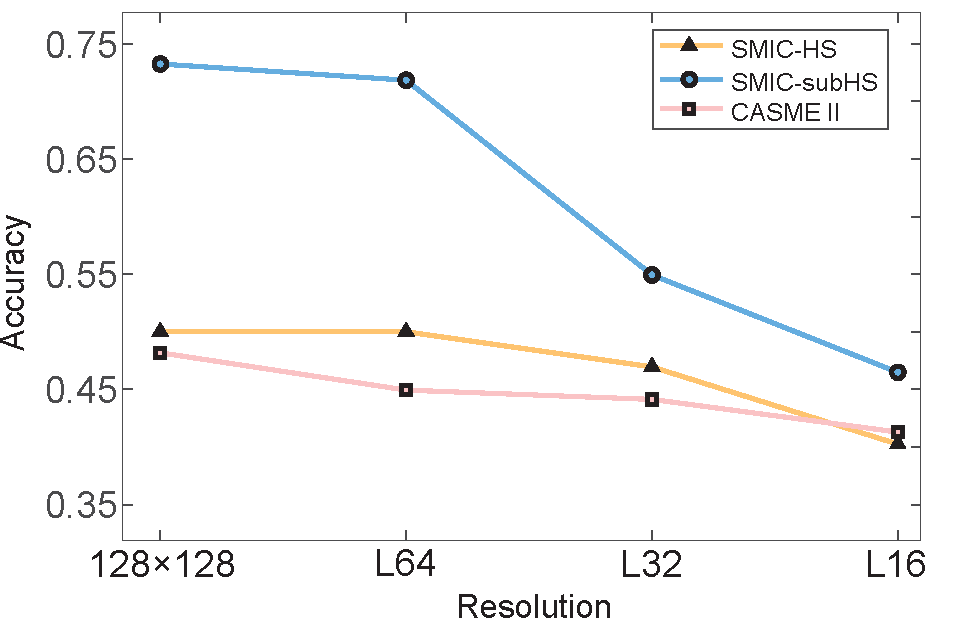
\includegraphics[width=0.60\textwidth]{LR6}
\caption{不同数据集不同分辨率的图像序列的识别准确度}
\label{fig16}
\end{figure}

图9为低分辨率图像序列分类结果的混淆矩阵,并以$ 128 \times 128 $分辨率下的性能为参考。我们可以发现,在SMICSubHS数据集(图9第二列)中,当图像序列的分辨率为$ 128 \times 128 $时,混淆矩阵更加集中在对角线上,说明微表情识别方法的识别效果较好。然而,当图像序列的分辨率降低时,混淆矩阵逐渐变差。我们还可以发现,在SMICHS(图9第一列)和CASME II(图9第三列)中,误分类的比例大于SMICsubHS,图8所示的识别准确率也相对较低。对于SMIC-HS来说,上述问题的主要原因可能是后8个受试者(SMIC-subHS数据集)的分布比前8个受试者更加均衡。对于CASME II来说,主要是由于分布不平衡和类别过多。例如,在CASME II数据集中,来自类other的视频片段数量占40.08\%。

\begin{figure}[!htb]
\centering
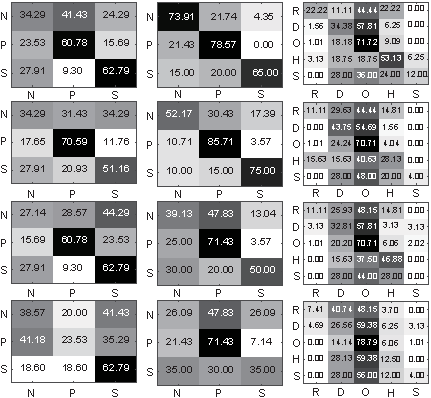
\includegraphics[width=0.75\textwidth]{LR7}
\caption{不同分辨率图像序列的识别准确度混淆矩阵}
\label{fig17}
\end{figure}

水平方向,从左往右依次是SMIC-HS数据集、SMIC-subHS数据集和CASME II数据集。垂直方向,从上到下依次是$ 128 \times 128 $分辨率混淆矩阵、$ 64 \times 64 $分辨率混淆矩阵、$ 32 \times 32 $分辨率混淆矩阵和 $ 16 \times 16 $。其中P代表积极(positive)、N代表消极(negative)、S代表惊喜(surprise)、R代表蔑视(repression)、D代表沮丧(disgust)、O代表其他(others)、H代表开心(happiness)。

在本小节中,我们将在三个数据集上对我们提出的框架进行实验。首先将测试集重构为$ 128 \times 128 $的分辨率,然后在高分辨率空间中进行分类。通过实证分析,选择了最优参数。表4给出了识别精度以及相应的块大小参数设置。从表4可以看出,实验结果有了显著的改善。例如在SMIC-subHS数据集中,$ 64 \times 64 $分辨率下的图像序列识别准确率从71.83\%提高到74.65\%,提高了2.82\%。S32的识别准确率为74.65\%,比L32高19.72\%。S16的识别准确率为73.24\%,比L16高26.76\%。这表明该方法对低分辨率图像序列的微表情识别精度有较好的提高。我们还注意到,与直接将输入作为原始的128128个图像序列相比,该框架使用S64得到了更好的结果。这可能是因为原始SMIC-HS/subHS数据集中的样本在记录过程中存在明显的噪声,使得人脸序列实际上包含了冗余和噪声信息。

超分辨率重建图像序列识别精度的混淆矩阵如图~\ref{fig17}所示。我们展示了$ 128 \times 128 $、S64、S32和S16图像序列根据不同数据集的识别精度。从图~\ref{fig17}可以看出,我们提出的框架的混淆矩阵比图9更集中在对角线上。特别是在$ 16 \times 16 $ SMIC-HS数据集(左下),积极的识别精度有显著提高。此外,我们可以从SMIC-subHS数据集(第二列)的结果中看出,将阴性误分类为阳性的比例显著降低,而将阳性正确分类的比例也得到了大幅提高。不幸的是,尽管CASME II数据集(第三列)的结果有所改善,但每个类别的分类仍然很差,通常错误地划分为其他类别。也许是因为其他微表情包含了所有其他类型的微表情,不包括惊讶、快乐、厌恶和压抑,所以它的分类是混合的。综上所述,从图~\ref{fig17}和图9的对比中我们可以看出,该框架对于低分辨率的微表情识别具有很好的性能提升。

\begin{table}[!htb]
\centering
\caption{不同分辨率图像在不同数据集上的识别精度比较}
\label{tab7}
\scalebox{0.81}{
\renewcommand{\arraystretch}{1.4}
\begin{tabular}{c|c|ccc|ccc}
\hline
\multirow{2}{*}{Accuracy (\%)} & High-resolution & \multicolumn{3}{c|}{Super-resolution Reconstruction} & \multicolumn{3}{c}{Low-resolution} \\ \cline{2-8}
 & $ 128 \times 128 $ & $ 64 \times 64 $ & $ 32 \times 32 $ & $ 16 \times 16 $ & $ 64 \times 64 $ & $ 32 \times 32 $ & $ 16 \times 16 $ \\ \hline
SMIC-HS & \begin{tabular}[c]{@{}c@{}}50.00\\ ($ 8 \times 8 \times 2 $)\end{tabular} & \begin{tabular}[c]{@{}c@{}}52.44\\ ($ 5 \times 5\times 2 $)\end{tabular} & \begin{tabular}[c]{@{}c@{}}51.83\\ ($ 5 \times 5 \times 2 $)\end{tabular} & \begin{tabular}[c]{@{}c@{}}51.83\\ ($ 5 \times 5 \times 2 $)\end{tabular} & \begin{tabular}[c]{@{}c@{}}50.00\\ ($ 6 \times 6 \times 5 $)\end{tabular} & \begin{tabular}[c]{@{}c@{}}46.95\\ ($ 6 \times 6 \times 5 $)\end{tabular} & \begin{tabular}[c]{@{}c@{}}40.24\\ ($ 3 \times 3 \times 6 $)\end{tabular} \\
SMIC-subHS & \begin{tabular}[c]{@{}c@{}}73.24\\ ($ 5 \times 5 \times 2 $)\end{tabular} & \begin{tabular}[c]{@{}c@{}}74.65\\ ($ 5\times 5 \times 2 $)\end{tabular} & \begin{tabular}[c]{@{}c@{}}74.65\\ ($ 5 \times 5 \times 2 $)\end{tabular} & \begin{tabular}[c]{@{}c@{}}73.24\\ ($ 8 \times 8 \times 3 $)\end{tabular} & \begin{tabular}[c]{@{}c@{}}71.83\\ ($ 6 \times 6 \times 2 $)\end{tabular} & \begin{tabular}[c]{@{}c@{}}54.93\\ ($ 6 \times 6 \times 2 $)\end{tabular} & \begin{tabular}[c]{@{}c@{}}46.48\\ ($ 4 \times 4 \times 1 $)\end{tabular} \\
CASME II & \begin{tabular}[c]{@{}c@{}}48.18\\ ($ 7 \times 7 \times 3 $)\end{tabular} & \begin{tabular}[c]{@{}c@{}}48.18\\ ($ 7 \times 7 \times 5 $)\end{tabular} & \begin{tabular}[c]{@{}c@{}}44.53\\ ($ 7 \times 7 \times 3 $)\end{tabular} & \begin{tabular}[c]{@{}c@{}}42.92\\ ($ 7 \times 7 \times 5 $)\end{tabular} & \begin{tabular}[c]{@{}c@{}}44.94\\ ($ 7 \times 7 \times 1 $)\end{tabular} & \begin{tabular}[c]{@{}c@{}}44.13\\ ($ 4 \times 4 \times 2 $)\end{tabular} & \begin{tabular}[c]{@{}c@{}}41.30\\ ($ 2 \times 2 \times 5 $)\end{tabular} \\ \hline
\end{tabular} }
\end{table}

High-resolution是指分辨率为$ 128 \times 128 $的图像序列,Super-resolution Reconstruction是指将低分辨率图像序列通过超分辨率重建方法为$ 128 \times 128 $,Low-resolution是指重建前的低分辨率图像序列。$ \mathrm{X} \times \mathrm{Y}  \times \mathrm{T} $指水平、垂直和时间方向块的数量。

\section{总结}

This Chapter focuses on the studies of ME analysis. We first reviewed the state-of-the-art progress about ME studies, including psychological studies about the concept and phenomenon of the ME, the challenges of collecting ME data, earlier studies using posed MEs, and also more recent studies of automatic ME spotting and recognition using spontaneous ME datasets. Then four parts of works about spontaneous ME analysis done by us were introduced, including 1) the collection of the first spontaneous ME database SMIC; 2) a framework for ME recognition; 3) an ME spotting method using feature difference analysis; and 4) an automatic ME analysis system (MESR) for firstly spotting and then the recognition of MEs.
本章着重于ME分析的研究。我们首先回顾了ME研究的最新进展,包括关于ME的概念和现象的心理学研究、收集ME数据的挑战、早期使用所提出的MEs的研究,以及最近使用自发ME数据集进行ME自动定位和识别的研究。然后介绍了我们所做的关于自发ME分析的四部分工作,包括1)收集了第一个自发ME数据库SMIC;2)自我认知的框架;3)基于特征差异分析的ME定位方法;4)自动ME分析系统(MESR),用于先定位后识别MEs。

The topic of ME analysis concerns facial movements at a very fine level. It is at an early stage by now, but it is attracting more attentions and developing rapidly. New databases are emerging, and new methods have been proposed with better performance both for ME recognition and for ME spotting. In future computers might be able to sense people s hidden feelings better than us with the ability to accurately spot and recognize MEs. We were the first few researchers that devoted to this topic. The main contributions of our exploratory works are 1) to break the ground and attract more researchers to the topic of ME; 2) to provide data as a benchmark for future studies; and 3) to propose basic framework and possible solutions for countering ME-specific challenges (e.g., the short duration and the intensity of movements) that may inspire future work. I plan to continue research on ME analysis in future, and detailed plans is described in Section 4.
ME分析的主题是非常精细的面部运动。虽然目前还处于起步阶段,但已引起越来越多的关注,发展迅速。新的数据库正在出现,新的方法已经被提出,它们在ME识别和ME定位方面都有更好的性能。在未来,计算机可能比我们更好地感知人们隐藏的情感,并能准确地发现和识别MEs。我们是第一批致力于这一课题的研究人员。我们探索性工作的主要贡献是:1)开拓创新,吸引更多的研究者关注我的课题;2)提供数据作为未来研究的基准;3)提出基本框架和可能的解决方案,以应对可能激励未来工作的ME-specific挑战(如短期和运动强度)。我计划在未来继续对ME分析进行研究,具体计划见第4节。

本文对低分辨率微表情识别问题进行了全面的研究。我们使用模糊和下采样模型来生成和模拟低分辨率的微表情人脸图像序列。我们在每一帧上使用面部幻觉的方法重建高质量的面部图像序列,增强局部细节,将低质量的图像序列放大到高分辨率的图像序列。然后利用快速LBP-TOP提取动态特征,利用SVM分类器对微表情进行识别。实验结果表明,在低分辨率的微表情识别问题上,该框架在可公开获取的微表情数据集(SMIC-HS、SMIC-subHS、CASME II)上表现良好。未来,我们将重点研究低分辨率情况下微表情识别的深度特征。
